\documentclass[portrait,pstricks,fancybox,epsfig,colordvi,semcolor,semlayer,a4,rotate]{seminar}
\usepackage{epsfig}
\usepackage{amsmath}
\usepackage{rotating}
\newcommand{\DIFFVM}{{\sc diffVM}}
\newcommand{\QPM}{Quark--Parton--Modell}

\newcommand{\Zero}   {\mbox{$Z^{\circ}$}}
\newcommand{\Ftwo}   {\mbox{$F_2$}}
\newcommand{\Fz}   {\mbox{$F_3$}}
\newcommand{\FL}   {\mbox{$F_{_{L}}$}}
\newcommand{\Fem}  {\mbox{$F_2^{em}$}}
\newcommand{\Fint} {\mbox{$F_2^{int}$}}
\newcommand{\Fwk}  {\mbox{$F_2^{wk}$}}
\newcommand{\FtD}{\tilde{F}_2^D(\beta,Q^2)}
\newcommand{\flux}{f_{\pom/p}(\xpom,t)}
\newcommand{\ftild}{\tilde{F}_2^D}
\newcommand{\fd}[1]{\ensuremath{F_2^{D\,( #1)}}} 
\newcommand{\flp}[1]{\ensuremath{F_2^{LP\,( #1)}}} 
\newcommand{\flptilda}{\ensuremath{\tilde{F}_2^{LP}}}
\newcommand{\rd}[1]{\ensuremath{R_2^{D\,( #1)}}} 

\newcommand{\dsiget}{\ensuremath{{\rm d}\sigma_{\gamma^*p}/{\rm d}E_t^*} }
\newcommand{\dsigrap}{\ensuremath{{\rm d}\sigma_{\gamma^*p}/{\rm d}\eta^*} }

\newcommand{\Rp}{\mbox{$\not \hspace{-0.15cm} R_p$}}
\newcommand{\e}{{\mathrm {e}}}
\newcommand{\dstar}{D^{* \pm}}
%\newcommand{\do}{D^0}
\newcommand{\slowpi}{\pi^{\pm}_{slow}}
\newcommand{\kpm}{K^{\pm}}
\newcommand{\dobar}{\bar{D}^0}
\newcommand{\pipm}{\pi^{\pm}}
\newcommand{\PO}{{\rm l \! P }}
\newcommand{\vrho}{\mbox{$\varrho$}}
\newcommand{\rhz}{\mbox{$\rh^0$}}
\newcommand{\ph}{\mbox{$\phi$}}
\newcommand{\om}{\mbox{$\omega$}}
\newcommand{\jpsi}{\mbox{$J/\psi$}}
\newcommand{\rzzziz}{\mbox{$r_{00}^{04}$}}
\newcommand{\ppi}{\pi}
\newcommand{\ii}{{\mathrm i}}
\newcommand{\odd}{Odd.}

\newcommand{\xpi}{\ensuremath{x_\ppi}}
\newcommand{\xbj}{x_{Bj}}
\newcommand{\pt}{p_{_T}}
\newcommand{\ptt}{P_T^{*2}}
\newcommand{\et}{\ensuremath{E_t^*} }
\newcommand{\QQ}{\mbox{${Q^2}$}}
%\newcommand{\Q4}{\mbox{${Q^4}$}}
\newcommand{\Qsq}{\mbox{$Q^2$}}
\newcommand{\qsq}{\mbox{$Q^2$}}
\newcommand{\W}{\mbox{$W$}}
\newcommand{\x}{\mbox{$x$}}
\newcommand{\y}{\mbox{$y$}}
\newcommand{\ttr}{\mbox{$t$}}
\newcommand{\tmin}{{\ensuremath{t_\mathrm{min}}}}
\newcommand{\tmax}{{\ensuremath{t_\mathrm{max}}}}
\newcommand{\s}{\mbox{$s$}}
\newcommand{\R}{\mbox{$R$}}
\newcommand{\bslope}{\mbox{$b$}}
\newcommand{\eclmax}{\mbox{$E_{max}$}}
\newcommand{\eminpz}{\mbox{$E-p_z$}}
\newcommand{\costhst}{\mbox{$\cos\theta^*$}}
\newcommand{\etamax}{\mbox{$\eta_{\rm max}\; $}}
\newcommand{\rap}{\ensuremath{\eta^*} }


\newcommand{\Wgp}{W_{\gamma p}}
\newcommand{\avWgp}{\langle\Wgp\rangle}
\newcommand{\xpom}{x_{_{\rm I\!P}}}
\newcommand{\modt}{\mid\!t\!\mid}
\newcommand{\gapprox}{\stackrel{>}{_{\sim}}}
\newcommand{\lapprox}{\stackrel{<}{_{\sim}}}
\newcommand{\pom}{\rm I\!P}
\newcommand{\reg}{\rm I\!R}
\newcommand{\mx}{M_{_X}}
\newcommand{\my}{M_{_Y}}
\newcommand{\yda}{y_{_{\it DA}}}
\newcommand{\yjb}{y_{_{\it h}}}
\newcommand{\ysig}{y_{_{\Sigma}}}
\newcommand{\qssig}{Q^2_{_{\Sigma}}}
\newcommand{\alphapom}{\alpha_{_{\rm I\!P}}}
\newcommand{\alphareg}{\alpha_{_{\rm I\!R}}}
\newcommand{\alpham}{\alpha_{_{\rm M}}}
\newcommand{\alphamt}{\alpha_{_{\rm M2}}}
\newcommand{\ftpom}{F_2^{^{\rm I\!P}}(\beta,Q^2)}
\newcommand{\ftreg}{F_2^{^{\rm I\!R}}(\beta,Q^2)}
\newcommand{\fpom}{f_{_{{\rm I\!P}/p}}(\xpom,t)}
\newcommand{\fpomnt}{f_{_{{\rm I\!P}/p}}(\xpom)}
\newcommand{\fregnt}{f_{_{{\rm I\!R}/p}}(\xpom)}
\newcommand{\fint}{f^{I}(\xpom)}
\newcommand{\npom}{n_{_{\rm I\!P}}}
\newcommand{\nreg}{n_{_{\rm I\!R}}}
\newcommand{\bpom}{B_{_{\rm I\!P}}}
\newcommand{\bm}{B_{_{\rm M}}}
\newcommand{\breg}{B_{_{\rm I\!R}}}
\newcommand{\etamin}{\eta_{\rm min}^Y}
\newcommand{\dthreesig}{\frac{{\rm d}^3 \sigma^D_{e p \rightarrow e X
    Y}}{{\rm d}x \,{\rm d}\beta\,{\rm d}Q^2}}
\newcommand{\dthreesigb}{\frac{{\rm d}^3 \sigma^D}{{\rm d}x \,{\rm d}\beta\,{\rm d}Q^2}}
\newcommand{\ftdt}{F_2^{D(3)}(\xpom,\beta,Q^2)}
\newcommand{\ftdtb}{F_2^{D(3)}}
\newcommand{\ftdf}{F_2^{D(4)}(\xpom,\beta,Q^2,t)}
\newcommand{\ft}{F_2(x,Q^2)}
\newcommand{\fl}{F_L(x,Q^2)}
\newcommand{\dtwosig}{\frac{{\rm d}^2 \sigma }{{\rm d}x\,{\rm d}Q^2}}

\newcommand{\mpipi}{\mbox{$m_{\pi^+\pi^-}$}}
\newcommand{\mll}{\mbox{$m_{l^+l^-}$}}
\newcommand{\mpp}{\mbox{$m_{\pi\pi}$}}      
\newcommand{\mppsq}{\mbox{$m_{\pi\pi}^2$}}  
\newcommand{\mpi}{\mbox{$m_{\pi}$}}         
\newcommand{\mrho}{\mbox{$m_{\rho}$}}       
\newcommand{\mrhosq}{\mbox{$m_{\rho}^2$}}   

\newcommand{\pp}{\mbox{$p\bar{p}$}}
\newcommand{\qq}{\mbox{$q\bar{q}$}}
\newcommand{\ep}{\mbox{$ep$}}
\newcommand{\gs}{\mbox{$\gamma^*$}}
\newcommand{\gsp}{\mbox{$\gamma^* p$}}
\newcommand{\gpcms}{\gamma^* \, \pom}
\newcommand{\Gmpp}{\mbox{$\Gamma (\mpp)$}}  
\newcommand{\Gmppsq}{\mbox{$\Gamma^2(\mpp)$}}
\newcommand{\Grho}{\mbox{$\Gamma_{\rho}$}}   
\newcommand{\gp}{\mbox{$\gamma p$}}
\newcommand{\zin}{\mbox{${\rm z_\Psi}$}}
\newcommand{\erho}{ep\to e\;\rho\;p}
\newcommand{\epsi}{ep\to e\;\jpsi\;p}
\newcommand{\ephi}{ep\to e\;\phi\;p}
\newcommand{\pipi}{\pi^+\pi^-}
\newcommand{\KK}{K^+K^-}

\newcommand{\llq}{$\alpha_s \ln{(\qsq / \Lambda_{QCD}^2)}$}
\newcommand{\llqx}{$\alpha_s \ln{(\qsq / \Lambda_{QCD}^2)} \ln{(1/x)}$}
\newcommand{\llx}{$\alpha_s \ln{(1/x)}$}

\newcommand{\MeV}{\mathrm{MeV}}
\newcommand{\gev}{\mbox{\rm GeV}}
\newcommand{\gevc}{\mbox{\rm GeV/c}}
\newcommand{\GeV}{\mbox{\rm GeV}}
\newcommand{\TeV}{{\rm TeV}}
\newcommand{\geVx}{\rm GeV}
\newcommand{\GeVsq}{\mbox{${\rm GeV}^2$}}
\newcommand{\gevsq}{\mbox{${\rm GeV}^2$}}
\newcommand{\gevsqc}{\mbox{${\rm GeV^2/c^4}$}}
\newcommand{\gevcsq}{\mbox{${\rm GeV/c^2}$}}
\newcommand{\mevcsq}{\mbox{${\rm MeV/c^2}$}}
\newcommand{\GeVsqm}{\mbox{${\rm GeV}^{-2}$}}
\newcommand{\gevsqm}{\mbox{${\rm GeV}^{-2}$}}

\newcommand{\nb}{\mathrm{nb}}
\newcommand{\pb}{\mathrm{pb}}
\newcommand{\ub}{\ensuremath{\mathrm{\mu b}}}
\newcommand{\nbinv}{\mbox{${\rm nb^{-1}}$}}
\newcommand{\pbinv}{\mbox{${\rm pb^{-1}}$}}

\newcommand{\us}{\ensuremath{\mathrm{\mu s}}}
\newcommand{\um}{\ensuremath{\mathrm{\mu m}}}
\newcommand{\cm}{\mathrm{cm}}
\newcommand{\m}{\mathrm{m}}
\newcommand{\mm}{\mathrm{mm}}
\newcommand{\urad}{\ensuremath{\mathrm{\mu rad}}}
\newcommand{\mrad}{\mathrm{mrad}}
\newcommand{\rad}{\mathrm{rad}}
\newcommand{\degree}{^\circ}
    
\newcommand{\BPC}{{\rm BPC}}    
\newcommand{\BEMC}{{\rm BEMC}}  
\newcommand{\lAr}{{\rm lAr}}    
\newcommand{\Had}{{\rm Had}}    
\newcommand{\had}{{\rm had}}    

\newcommand{\BR}{\mathit{BR}}
\newcommand{\der}{{\mathrm d}}
\newcommand{\md}{\mbox{d}}
\newcommand{\average}[1]{\mbox{$ \langle #1 \rangle $}}
\newcommand{\av}[1]{\mbox{$ \langle #1 \rangle $}}
\newcommand{\lsim}{\raisebox{-0.5mm}{$\stackrel{<}{\scriptstyle{\sim}}$}}
\newcommand{\gsim}{\raisebox{-0.5mm}{$\stackrel{>}{\scriptstyle{\sim}}$}}
\newcommand{\stat}{{\rm stat.}}
\newcommand{\syst}{{\rm syst.}}

\newcommand{\hdick}{\noalign{\hrule height1.4pt}}
\newcommand{\hs}[1]{\hspace{#1ex}}
\newcommand{\anglearrow}{^|\hspace{-0.5em}\rightarrow}
\newcommand {\sub}[1]{\ensuremath{_{\mathrm{#1}}}} 
\newcommand{\scaption}[1]{\caption{\protect{\footnotesize  #1}}}
\newcommand{\proc}[2]{\mbox{$ #1 \rightarrow #2 $}}
\newcommand{\rb}[1]{\raisebox{2mm}[-2mm]{#1}}
\newcommand {\rh}[0]{\rule[-3mm]{0cm}{10mm}}
\newcommand\bs{\char '134}
\newcommand{\nodel}[1]{\multicolumn{1}{c}{#1}}
\newcommand {\unit} [1] {\mathrm {#1}}

\newcommand{\Brodsky}{Brodsky {\it et al.}}
\newcommand{\FKS}{Frankfurt, Koepf and Strikman}
\newcommand{\Kop}{Kopeliovich {\it et al.}}
\newcommand{\Ginzburg}{Ginzburg {\it et al.}}
\newcommand{\Ryskin}{\mbox{Ryskin}}
\newcommand{\Kaidalov}{Kaidalov {\it et al.}}


\newcommand {\zit}[7]
 {\bibitem[#1]{#2}{\scshape #3} {\upshape #4 (#5): #6 ---} {\itshape #7}}
\newcommand {\zitcol}[7]{\zit{#1}{#2}{{\upshape #3}, #4}{et al.}{#5}{#6}{#7}}
\newcommand {\zitz}[4]{#1 {\bfseries #2}, #3.}
\newcommand {\zitzn}[5]{#1 {\bfseries #2} (No. #3), #4.}
\newcommand {\zitibid}[2]{ibid. {\bfseries #1}, #2.}
\newcommand {\zitibidn}[3]{ibid. {\bfseries #1} (No. #2), #3.}
%\newcommand {\zitz}[4]{#1 {\bfseries #2}, #3, #4.}
%\newcommand {\zitzn}[5]{#1 {\bfseries #2} (No. #3), #4, #5.}
%\newcommand {\zitp}[3]{#1, #3.}
\newcommand {\zitp}[3]{#1, #2\,pp., #3.}
\newcommand {\zitnp}[2]{\zitz{Nucl. Phys.}{#1}{#2}{Amsterdam}}
\newcommand {\zitnpn}[3]{\zitzn{Nucl. Phys.}{#1}{#2}{#3}{Amsterdam}}
\newcommand {\zitplx}[2]{\zitz{Phys. Lett.}{#1}{#2}{Amsterdam}}
\newcommand {\zitpl}[3]{\zitzn{Phys. Lett.}{#1}{#2}{#3}{Amsterdam}}
\newcommand {\zitprep}[3]{\zitzn{Phys. Rep.}{#1}{#2}{#3}{Amsterdam}}
\newcommand {\zitnim}[2]{\zitz{Nucl. Instr. Meth. Phys. Res.}{#1}{#2}{Amsterdam}}
\newcommand {\zitpr}[3]{\zitzn{Phys. Rev.}{#1}{#2}{#3}{Lancaster, PA}}
\newcommand {\zitprx}[2]{\zitz{Phys. Rev.}{#1}{#2}{Lancaster, PA}}
\newcommand {\zitprd}[3]{\zitzn{Phys. Rev.}{#1}{#2}{#3}{Woodbury, NY}}
\newcommand {\zitprdx}[2]{\zitz{Phys. Rev.}{#1}{#2}{Woodbury, NY}}
\newcommand {\zitprl}[3]{\zitzn{Phys. Rev. Lett.}{#1}{#2}{#3}{New York, NY}}
\newcommand {\zitzp}[2]{\zitz{Z. Phys.}{#1}{#2}{Berlin}}
\newcommand {\zitzpn}[3]{\zitzn{Z. Phys.}{#1}{#2}{#3}{Berlin}}

\newcommand {\zitb}[3]{#1\,pp., #2 (#3).}
\newcommand {\zitbd}[3]{#1\,S., #2 (#3).}
\newcommand {\zitc}[2]{CERN preprint #1, #2\,pp., Geneva.}
\newcommand {\zitd}[2]{DESY report #1, #2\,pp., Hamburg.}
\newcommand {\zite}[1]{Electronic preprint {\bfseries #1.}}
\newcommand {\zith}[2]{H1 internal report #1, #2\,pp., unpublished.}

\newcommand {\herawsi}
 {{\sc Peccei, R.\,D. }{\rm (ed.) (1988):
  Proceedings of the HERA workshop. Hamburg, October 12--14, 1987. ---}
  {\it iv+937\,pp., 2 vols., Hamburg (DESY)}}
\newcommand {\herawsii}
 {{\sc Buchm\"uller, Wilfried \& G. Ingelman }{\rm (eds.) (1992):
  Proceedings of the workshop Physics at HERA. Hamburg,
  October 29--30, 1991. ---}
  {\it xiv+1566\,pp., 3 vols., Hamburg (DESY)}}









\newrgbcolor{darkgreen}{0 0.5 0}
\newrgbcolor{darkblue}{0 0 0.5}
\newrgbcolor{lightgreen}{0 0.7 0}
\newrgbcolor{darkred}{0.7 0 0}

\newcmykcolor{GreenYellow}{0.15 0  0.69 0 } 
\newcmykcolor{Yellow}{0 0 1 0 }  
\newcmykcolor{Goldenrod}{0 0.10 0.84 0 } 
\newcmykcolor{Dandelion}{0 0.29 0.84 0 }  
\newcmykcolor{Apricot}{0 0.32 0.52 0} 
\newcmykcolor{Peach}{0 0.50 0.70 0 }  
\newcmykcolor{Melon}{0 0.46 0.50 0 }  
\newcmykcolor{YellowOrange}{0 0.42 1 0 }  
\newcmykcolor{Orange}{0 0.61 0.87 0 }  
\newcmykcolor{BurntOrange}{0 0.51 1 0 } 
\newcmykcolor{Bittersweet}{0 0.75 1 0.24 }   
\newcmykcolor{RedOrange}{0 0.77 0.87 0 }  
\newcmykcolor{Mahogany}{0 0.85 0.87 0.35 }  
\newcmykcolor{Maroon}{0 0.87 0.68 0.32 }  
\newcmykcolor{BrickRed}{0 0.89 0.94 0.28 } 
\newcmykcolor{Red}{0 1 1 0 }  
\newcmykcolor{OrangeRed}{0 1 0.50 0 } 
\newcmykcolor{RubineRed}{0 1 0.13 0 }  
\newcmykcolor{WildStrawberry}{0 0.96 0.39 0 }     
\newcmykcolor{Salmon}{0 0.53 0.38 0 }  
\newcmykcolor{CarnationPink}{0 0.63 0 0 }  
\newcmykcolor{Magenta}{0 1 0 0 }  
\newcmykcolor{VioletRed}{0 0.81 0 0 }  
\newcmykcolor{Rhodamine}{0 0.82 0 0 }  
\newcmykcolor{Mulberry}{0.34 0.90 0 0.02 }  
\newcmykcolor{RedViolet}{0.07 0.90 0 0.34}  
\newcmykcolor{Fuchsia}{0.47 0.91 0 0.08 }  
\newcmykcolor{Lavender}{0 0.48 0 0 }  
\newcmykcolor{Thistle}{0.12 0.59 0 0 }  
\newcmykcolor{Orchid}{0.32 0.64 0 0 }  
\newcmykcolor{DarkOrchid}{0.40 0.80 0.20 0} 
\newcmykcolor{Purple}{0.45 0.86 0 0 }  
\newcmykcolor{Plum}{0.50 1 0 0 } 
\newcmykcolor{Violet}{0.79 0.88 0 0 }  
\newcmykcolor{RoyalPurple}{0.75 0.90 0 0 }  
\newcmykcolor{BlueViolet}{0.86 0.91 0 0.04 }   
\newcmykcolor{Periwinkle}{0.57 0.55 0 0 }  
\newcmykcolor{CadetBlue}{0.62 0.57 0.23 0 } 
\newcmykcolor{CornflowerBlue}{0.65 0.13 0 0 }   
\newcmykcolor{MidnightBlue}{0.98 0.13 0 0.43 }    
\newcmykcolor{NavyBlue}{0.94 0.54 0 0 } 
\newcmykcolor{RoyalBlue}{1 0.50 0 0 }  
\newcmykcolor{Blue}{1 1 0 0 } 
\newcmykcolor{Cerulean}{0.94 0.11 0 0 }  
\newcmykcolor{Cyan}{1 0 0 0 } 
\newcmykcolor{ProcessBlue}{0.96 0 0 0 }  
\newcmykcolor{SkyBlue}{0.62 0 0.12 0 }  
\newcmykcolor{Turquoise}{0.85 0 0.20 0 }  
\newcmykcolor{TealBlue}{0.86 0 0.34 0.02 }  
\newcmykcolor{Aquamarine}{0.82 0 0.30 0 } 
\newcmykcolor{BlueGreen}{0.85 0 0.33 0 }  
\newcmykcolor{Emerald}{1 0 0.50 0}  
\newcmykcolor{JungleGreen}{0.99 0 0.52 0 }  
\newcmykcolor{SeaGreen}{0.69 0 0.50 0 }  
\newcmykcolor{Green}{1 0 1 0 } 
\newcmykcolor{ForestGreen}{0.91 0 0.88 0.12 }  
\newcmykcolor{PineGreen}{0.92 0 0.59 0.25 }  
\newcmykcolor{LimeGreen}{0.50 0 1 0 }  
\newcmykcolor{YellowGreen}{0.44 0 0.74 0 }  
\newcmykcolor{SpringGreen}{0.26 0 0.76 0 } 
\newcmykcolor{OliveGreen}{0.64 0 0.95 0.40 }  
\newcmykcolor{RawSienna}{0 0.72 1 0.45 }  
\newcmykcolor{Sepia}{0 0.83 1 0.70 }  
\newcmykcolor{Brown}{0 0.81 1 0.60 }  
\newcmykcolor{Tan}{0.14 0.42 0.56 0 }  
\newcmykcolor{Gray}{0 0 0 0.50 }  
\newcmykcolor{White}{0 0 0 0 } 

        

%
%--- Slide options
%
\centerslidestrue
\extraslideheight{10in}
\slidesmag{3}
\slidewidth 25cm
\slideheight 18.5cm
\slideframe{none}
\renewcommand{\slidefuzz}{2.5cm}
\renewcommand{\slidestretch}{1.}
\renewcommand{\slidetopmargin}{0.0in}
%
%--- Header lines
%
\newcommand{\header}[1]{
{\red
\begin{center}
\setlength{\arrayrulewidth}{1mm}
\setlength{\tabcolsep}{0mm}
\begin{tabular}{c}
{\huge \black #1} \\[0.6mm]
\hline
\end{tabular}
\end{center}}}

\newcommand{\bheader}[1]{
{\blue
\begin{center}
\setlength{\arrayrulewidth}{1mm}
\setlength{\tabcolsep}{0mm}
\begin{tabular}{c}
{\huge \black #1} \\[0.6mm]
\hline
\end{tabular}
\end{center}}}

\newcommand{\eheader}[1]{
{\red
\begin{center}
\setlength{\arrayrulewidth}{1mm}
\setlength{\tabcolsep}{0mm}
\begin{tabular}{c}
{\huge \black #1} \\[0.6mm]
\end{tabular}
\end{center}}}
%
\newcommand{\dd}{\displaystyle}
\newcommand{\hitb}{{\large\black $\bullet\;$}}
\newcommand{\hiti}{{\huge\blue $\bullet$}}
\newcommand{\iti}{{\Large\red $\bullet$}}
\newcommand{\itii}{{\darkgreen $\blacktriangleright$}}
\newcommand{\htab}{\rule[-1mm]{0mm}{6mm}}
\newcommand{\hhtab}{\rule[-5mm]{0mm}{12mm}}
%
%--- Pagestyle
%
\pagestyle{headings}
%\pagestyle{cern}
%\pagestyle{pssections}
%\pagestyle{empty}
%
%
%
\begin{document}
%
%
%

\begin{slide}
\pagestyle{headings}
\sf
\vspace*{-5mm} 
\header{Linear Least square fit - introductory example}
%
\large
\begin{center}
\begin{figure}[h]
\unitlength1cm
\begin{picture}(15.,10.)
\put(-1.,9.5){\begin{minipage}{6cm}
Example: Precise muon track fits for possible
discovery 
$Z^{*} \rightarrow \mu^{+} \mu^{-}$
\end{minipage}
}
\put(-1.,4.2){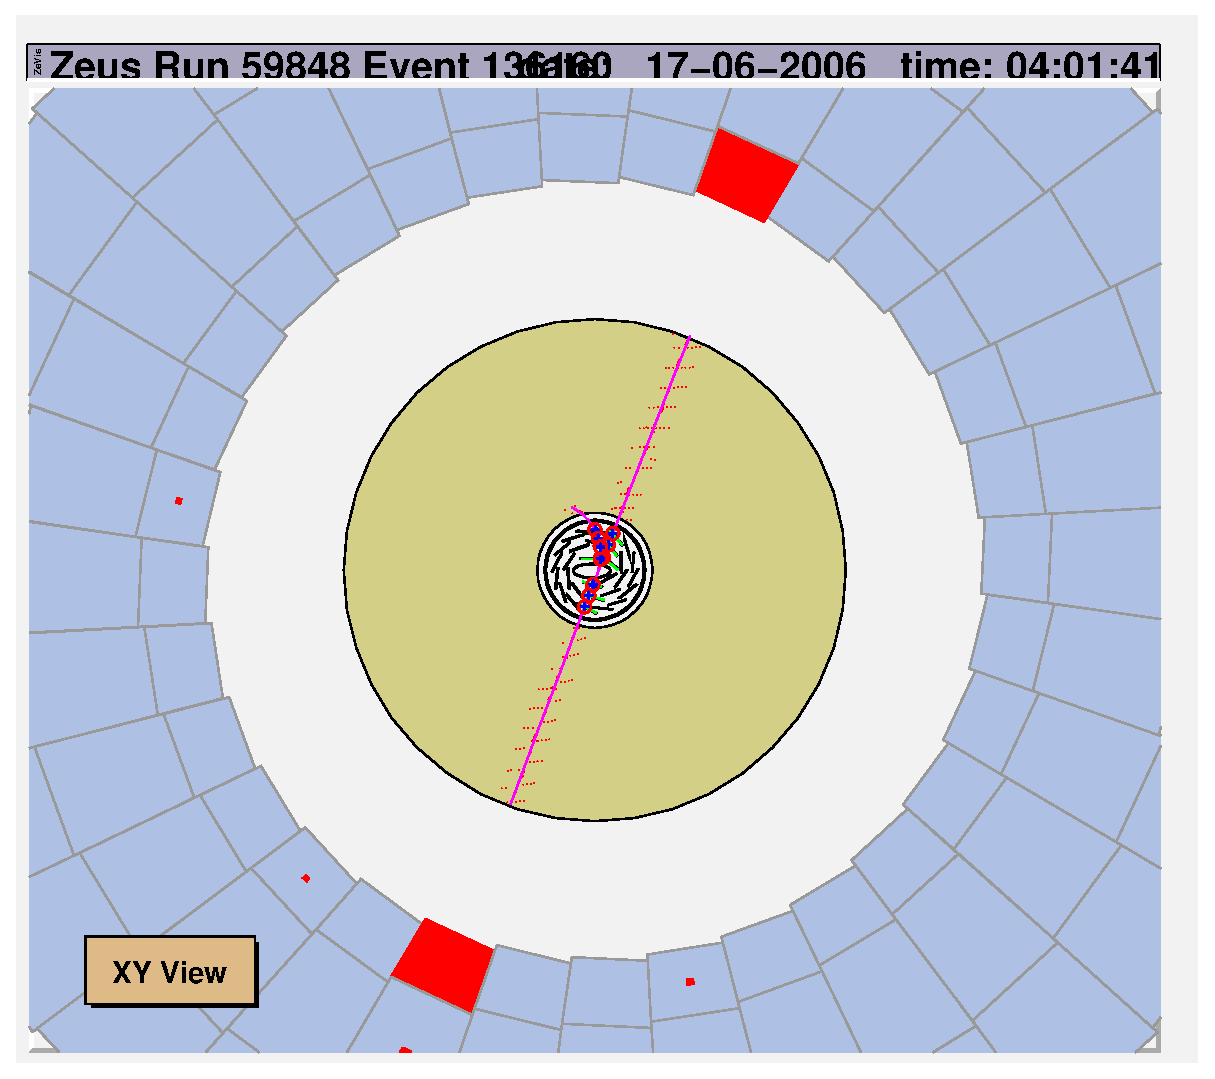
\epsfig{file=zevis/r59848e136160_trackcal_rphi.eps,width=5.5cm}}
\put(-1.3,-0.5){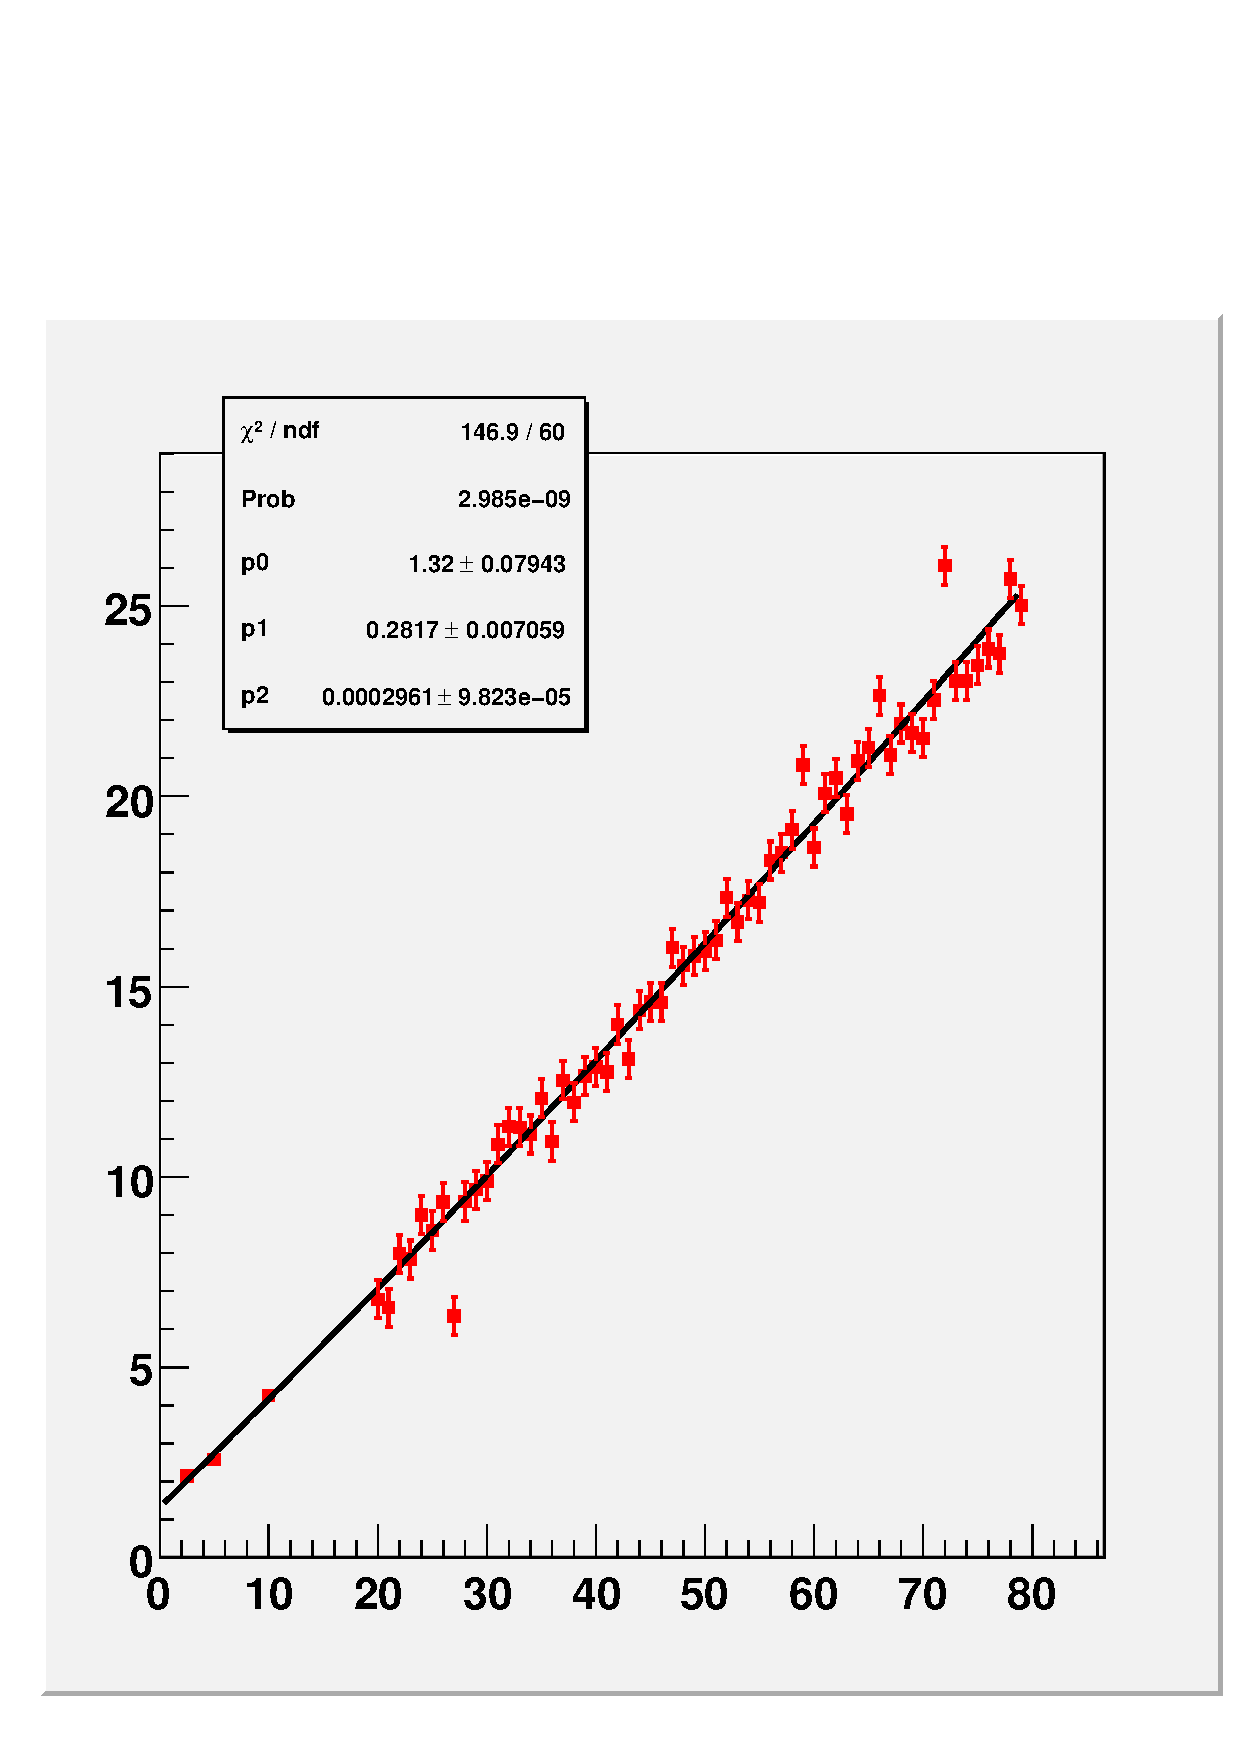
\epsfig{file=eps/trackfit.epsi,width=4.5cm}}
\put(1.5,1.){
\begin{minipage}{4.3cm}
\normalsize \it
Track example:
Detector measures
coordinate $y_i$ in n detector layers at fixed positions $x_i$
\end{minipage}
}
%
%
\put(6.,9.9){
\begin{minipage}[t]{8cm}
\normalsize
\begin{itemize}
\item
Necessary conditions for linear least square fit:
\begin{itemize}
\item
Measurements with gaussian uncertainties
\item
Linear model, here: $y = a_0 + a_1 x + a_2 x^2$
\end{itemize}
\item
Fit construction:
\begin{itemize}
\item
$\chi^2 = \sum_{i}
 \frac{\left[ y_i - (a_0 + a_1 x + a_2 x^2) \right]^2}{
\sigma_i^2}
$
\item
Determine $a_0, a_1, a_2$ by finding 
$\chi^2$ total minimum (normal equations)
\end{itemize}
\item
Check consistency
\begin{itemize}
\item
$\chi^2$ and fit probability
\item
Outlier rejection
\end{itemize}
\item
Detailed error analysis
\begin{itemize}
\item
Parameter errors and correlations (error ellipses),
%
%\item
track trajectory error band
\item
Momentum calculation (error propagation)
\end{itemize}
\item
Possible Extensions:
\begin{itemize}
\item
Apply constraint fits to both tracks, e.g. 
$p_t(\mu^{+}) = p_t(\mu^{-})$
{\red $\rightarrow$ covered in session on extended fits}
\item
Analysis of obtained $\mu^{+}\mu^{-}$ 
mass spectrum containing background and
possible signal events 
{\red $\rightarrow$ covered in session on non-linear least square fits}
%
%Reconstruct invariant mass $M(\mu^{+}\mu^{-}$,
%applying constra
\end{itemize}
\end{itemize}
\end{minipage}
}
\end{picture}
\end{figure}
\end{center}
\end{slide}
%
%



\begin{slide}
\pagestyle{headings}
\small
\sf 
\header{Overview of Linear least square fit section}
%\renewcommand{\arraystretch}{5.5}
\begin{table}
\setlength{\tabcolsep}{6pt}
\hspace*{-5mm}
\scriptsize
\begin{tabular}{|l|l|l|}
\hline
Part I & Part II & Part III \\
\hline
\begin{minipage}{3.6cm}
\vspace*{1mm}
%\begin{itemize}
\begin{list}{\labelitemi}{\leftmargin=1em}
\item
Reminder of $\chi^2$-fit method 
\item
Linear $\chi^2$-fit examples (Constant, straight
line, parabola, etc.)
\item
{\bfseries \blue Fit of a constant (averaging measurements)}
\item 
One single measurement:
$\chi^2_{min}$ and $\chi^2_{min}+1$,
Hesse matrix
\item
{\magenta Exercise: Two measurements:
perform fit by adding $\chi^2$-parabolas}
\item
Averaging many measurements, results
\item
 {\magenta Exercise: Compare
weighted vs unweighted average}
\end{list}
%\end{itemize}
\end{minipage}
&
\begin{minipage}{5.5cm}
\vspace*{1mm}
\begin{list}{\labelitemi}{\leftmargin=1em}
%\begin{itemize}
\item
{\blue \bfseries $\chi^2$-fit-quality test:}
Example: $\chi^2$ of two measurements
and known true value
\item
$\chi^2$-function for $n$ degrees of freedom
and $\chi^2$-fit probability
%\item
{\scriptsize \red Exercise: plot and study features
of the $\chi^2$-function vs $n$ using the parameterised function}
{\red New: Generate 1000 random experiments with n degrees of
freedom and obtain $\chi^2$ and $\chi^2$-fit probability distributions} 
%\item
%
%\item
%{\red exercise: 
%plot and study features
%of the $\chi^2$-fit-probability}
\item
$\chi^2$ for two measurements with unknown true value
\item
{\red \scriptsize New exercise: Track position measurement in test beam
using 10 detector layers, in each detector 99\%
chance for signal hit and 1\% for random noise hit
$\rightarrow$  Generate 1000 tracks and corresponding
hits and obtain $\chi^2$, $\chi^2$-fit probability 
and measured parameter distributions. 
Try to reject outliers: Method 1: reject track fits with
small $\chi^2$-fit probability, Method 2: iterative,
repeat track-fit and downweight outliers}
\item
{\red Exercise: {\blue \bfseries Outlier rejection}, case
world average of $m_W$, {\scriptsize  study how
the rejection of certain measurements 
change the average and the $\chi^2$-fit probability}}
\item
%{\scriptsize \darkgreen Averaging data with unknown errors}
%\item
{\red New exercise: Upscaling of errors a la PDG to obtain reasonable $\chi^2$}
\item
{\red New exercise: Pulls of single measurements to 
the average}
%\end{itemize}
\end{list}
\end{minipage}
& 
\begin{minipage}{5.cm}
\vspace*{1mm}
\begin{list}{\labelitemi}{\leftmargin=1em}
%\begin{itemize}
\item
General form of linear $\chi^2$
\item
Solution by normal equations
%\item
%General features:
%(Consistency, Unbiasedness, efficiency)
\item
Normal equation solution for 
{\blue \bfseries straight line
fit}
\item
{\magenta Exercise: Learn qualitative features
of straight line fits, e.g. importance of lever arm}
\item
{\red Exercise: Straight line fit and 
detailed error analysis (error ellipse, trajectory
error band)}
\item
{\red New exercise: Coordinate transformation such that the
coordinate center is in the middle of the points $\rightarrow$
study the effect on the parameter errors and correlation}
\item 
{\red New exercise: Add a very precise point at the origin of
the track such that the $p_0$ parameter is basically fixed.
Repeat the track-fit and study the effect on the slope and error}
\item
{\red Exercise: {\blue \bfseries Parabola track fit},
complete analysis: {\it \scriptsize fit, outlier-rejection, 
parameter errors/correlation, trajectory uncertainty,
{\blue \bfseries momentum calculation}}}
%\item
%{\red Exercise: {\blue \bfseries Guessing the right fit function
%for smooth data (polynomial fit of background}}
%\end{itemize}
\end{list}
\vspace*{1mm}
\end{minipage}
\\
\hline
\end{tabular}
\end{table}
\end{slide}

%\begin{slide}
\pagestyle{headings}
\sf 
\header{Method of least squares fit - a reminder}
%
\begin{center}
\unitlength1cm
\begin{figure}[h]
\unitlength1cm
\begin{picture}(15.,9.5)
\put(0.,0.){(0,0)}
\put(0.,2.){(0,2)}
\put(0.,4.){(0,4)}
\put(0.,6.){(0,6)}
\put(0.,8.){(0,8)}
\put(2.,0.){(2,0)}
\put(2.,2.){(2,2)}
\put(2.,4.){(2,4)}
\put(2.,6.){(2,6)}
\put(2.,8.){(2,8)}
\put(4.,0.){(4,0)}
\put(4.,2.){(4,2)}
\put(4.,4.){(4,4)}
\put(4.,6.){(4,6)}
\put(4.,8.){(4,8)}
\put(6.,0.){(6,0)}
\put(6.,2.){(6,2)}
\put(6.,4.){(6,4)}
\put(6.,6.){(6,6)}
\put(6.,8.){(6,8)}
\put(8.,0.){(8,0)}
\put(8.,2.){(8,2)}
\put(8.,4.){(8,4)}
\put(8.,6.){(8,6)}
\put(8.,8.){(8,8)}
\put(10.,0.){(10,0)}
\put(10.,2.){(10,2)}
\put(10.,4.){(10,4)}
\put(10.,6.){(10,6)}
\put(10.,8.){(10,8)}
\put(12.,0.){(12,0)}
\put(12.,2.){(12,2)}
\put(12.,4.){(12,4)}
\put(12.,6.){(12,6)}
\put(12.,8.){(12,8)}
\end{picture}
\end{figure}
\end{center}
\end{slide}

%
%
%

\begin{slide}
\pagestyle{headings}
\sf 
\header{Lecture I on linear least square fits}
%
\Large
Contents:
\begin{itemize}
\item
Least square $\chi^2$-fit method reminder
\item 
Linear least square fits: definition and examples
\item
Fit of a constant: One, two and many measurements
%
%\begin{itemize}
%\item One, two  measurement
%\item Two measurements..
%\item Many measurements...
%\end{itemize}
\end{itemize}
%
\end{slide}




%
%
%
\begin{slide}
\pagestyle{headings}
\sf 
\header{Method of least squares fit - a reminder}
%
\Large
\begin{center}
\begin{figure}[h]
\unitlength1cm
\begin{picture}(15.,9.5)
\put(0.,9.){\underline{Example problem: Particle trajectory measurement}}
\put(0.,2.3){\epsfig{file=feynman/l1.ps,width=6.cm}}
\put(7.,5.6){
\begin{minipage}{5cm}
\underline{general:}\\
$n$-measurements $y_i$ \\
with uncertainties $\sigma_i$\\
at fixed $x_i$\\
\underline{Model:} $ y=f(x,a)$
\end{minipage}
}
\put(0.,2){
\begin{minipage}[t]{13cm}
$\Rightarrow$ how to determine $a$?\\
Idea: for the correct $a$ one expects:
$|y_i - f(x_i,a)|\le \sigma_i$,\\
{\em i.e. curve describes data within 
measurement uncertainties}
\end{minipage}
}
\end{picture}
\end{figure}
\end{center}
\end{slide}
%
%
%
%
%
%
\begin{slide}
\pagestyle{headings}
\sf 
\header{Method of least squares fit - a reminder}
%
\Large
\begin{center}
\begin{figure}[h]
\unitlength1cm
\begin{picture}(15.,9.5)
%
\put(0.,8.){
$\rightarrow$ 
\mbox{\framebox{
$ \chi^2 = \Sigma_{i=1}^n \frac{ (y_i-f(x_i,a))^2}{\sigma_i^2} $}}
$\leftrightarrow \mbox{Minimum with respect to a}$
%\rightarrow \frac{d\chi^2}{da} = 0
%
}
\put(0.,6.5){
$\Rightarrow$ determine a from $\frac{d\chi^2}{da} = 0$
}
\put(0.,5.){
$\rightarrow$ 
\mbox{\framebox{
$ \frac{d\chi^2}{da} = \Sigma_{i=1}^n \frac{ (y_i-f(x_i,a))}{\sigma_i^2} 
\cdot \frac{df(x_i,a)}{da} = 0
$}}
}
\put(0.,3.5){
\begin{minipage}[t]{13cm}
In general not analytically solvable.\\
$\Rightarrow$ use iterative (numerical) methods
(MINUIT, Mathematica) 
\end{minipage}
}
\end{picture}
\end{figure}
\end{center}
\end{slide}


\begin{slide}
\pagestyle{headings}
\sf 
\header{Method of least squares fit - a reminder}
%
\Large
\begin{center}
\begin{figure}[h]
\unitlength1cm
\begin{picture}(15.,9.5)
%
\put(0.,9.){
\begin{minipage}[t]{8cm}
\underline{Most general case}\\
\begin{itemize}
\item  
$y_i,y_j$ correlated measurements with covariance $V_{ij}$
\item 
$m$ fitparameters $\vec{a}$
\end{itemize}
%\vspace*{1cm}
%
\[
\rightarrow
 \begin{array}{|lll|}
\hline
 \chi^2 &  = & \Sigma_{i,j=1}^n 
(y_i - f(x_i,\vec{a}))  V_{ij}^{-1} (y_j - f(x_j,\vec{a}))\\[2mm]
 & = & (\vec{y} - \vec{f}(\vec{a}))^t V^{-1} (\vec{y} - \vec{f}(\vec{a}))\\
\hline
\end{array}
\]
%
\end{minipage} 
%
}
\end{picture}
\end{figure}
\end{center}
\end{slide}




\begin{slide}
\pagestyle{headings}
\sf 
\header{Linear least square fits}
%
\Large
\begin{center}
\begin{figure}[h]
\unitlength1cm
\begin{picture}(15.,9.5)
\put(0.,8.){
\begin{minipage}[t]{15cm}
\Large
$\vec{y}\;$ vector of $n$ measurements
$\left( \begin{array}{l}
y_1(x_1)\\
. \\
y_n(x_n)\\
\end{array}
\right)
\;$
with cov-matrix $ V$\\
\vspace{5mm}

$ \vec{a}\;$ vector of m fitparameters 
$\left( \begin{array}{l}
a_1\\
. \\
a_m\\
\end{array}
\right)
$

%\vspace{2mm}
Model $\vec{y}: \;\; =   A \,\vec{a}$
%
\hspace{1cm}
\underline{Example:} $y=ax$; $\vec{a} = (a)$, 
$ 
A =
\left(
\begin{array}{l}
  x_1  \\
  . .  \\
  x_n  \\
 \end{array}
\right)
$
%\begin{center}
% 

%Master $\chi^2$:
$
\begin{array}{||l||}
\hline
\hline
\chi^2 = \left(\vec{y} - A \, \vec{a}\right)^t V^{-1}
            \left(\vec{y} - A \, \vec{a}\right)
%\quad
\\
\hline
\hline
\end{array}
$

\vspace{1mm}
$\rightarrow$ to be minimised w.r.t $\vec{a}$
%\end{center}
%
\end{minipage}
}
\end{picture}
\end{figure}
\end{center}
\end{slide}

%\begin{slide}
%\pagestyle{headings}
%\sf 
%\header{Examples for linear least square fits}
%%
%\Large
%\begin{itemize}
%\item
%Straight line fit $y_i =a x_i$, $\vec{a}=a$
%\[
%A =
%\left(
%\begin{array}{l}
%  x_1  \\
%  . .  \\
%  x_n  \\
% \end{array}
%\right)
%\]
%\end{itemize}
%\item 
%
%Watch out: linear in $\vec{a}$, 
%{\em but not necessarily in $x$}.\\
%Example fct =  $a e^{-x}$, i.e. model for $y_i$: =   $e^{-x_i}\, a$
%\vspace*{-2mm}
%\end{itemize}
%\end{slide}




\begin{slide}
\pagestyle{headings}
\sf 
\header{Examples for linear least square fits}
\begin{center}
{\em \normalsize Linear means that
$y$ depends linearly on the fitparameters $a_i$.}
\begin{figure}[h]
\unitlength1cm
\begin{picture}(15.,9.5)
%
    \put(1.,-.5){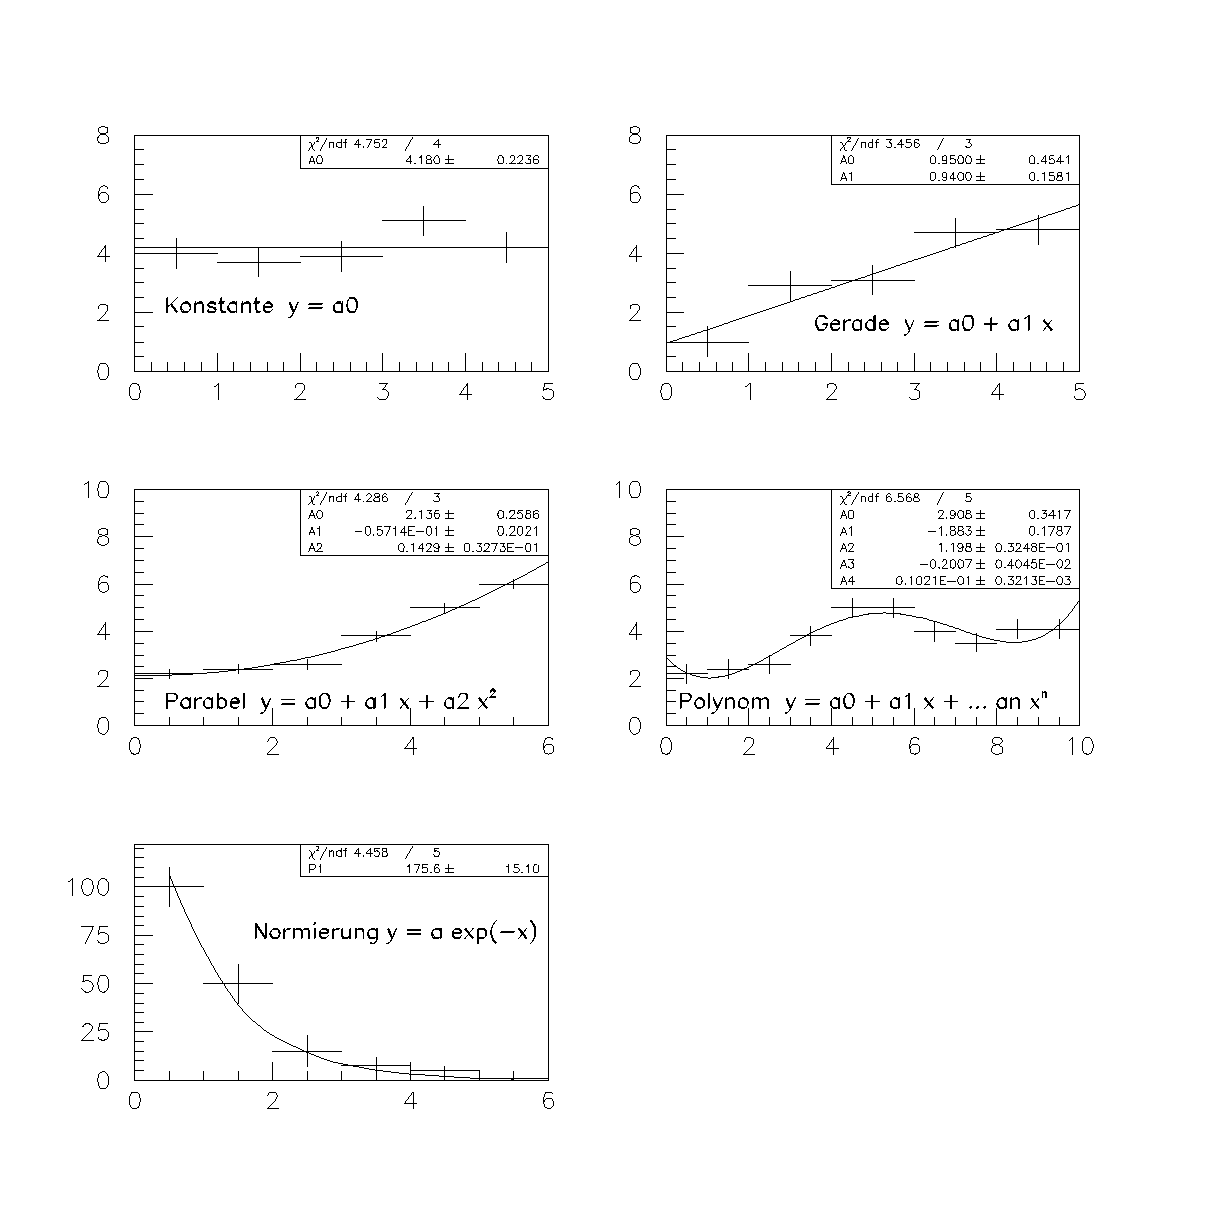
\epsfig{file=eps/linfits.eps,width=11.cm}}
\put(6.,1.){$\leftarrow$ 
\begin{minipage}[t]{5cm}
\em Watch out: function can be highly non-linear in $x$
\end{minipage}
}
\end{picture}
\end{figure}
\end{center}
\end{slide}
%
%
%





\begin{slide}
\pagestyle{headings}
\sf 
\header{Fit of a constant}
%\begin{center}
\vspace*{2mm}
\Large 
Example: Averaging of $n$ different measurements 
$a_i \pm \sigma_i$ of an observable $a$ (e.g. $a = \alpha_s(m_Z)$)
\[ \chi^2 = \Sigma_i^n \frac{ (a_i - a)^2}{\sigma_i^2} \]
``Idiot example'' of one single measurement $a_1 \pm \sigma_1$:
\[ \chi^2 = \frac{ (a_1 - a)^2}{\sigma_1^2} \]
\[Min. \chi^2: \quad \frac{d \chi^2}{da} = 0 \; 
\rightarrow \; \mbox{Estimated value}\quad
\hat{a} = a_1; \; \sigma_{\hat{a}} = \sigma_1 \]
%
%\end{center}
\end{slide}
%
%
%
%
\begin{slide}
\pagestyle{headings}
\sf 
\header{Fit of a constant {\em (single measurement)}}
\Large 
Probability density $p$ for true value of $a$ ({\em inverse probability}):
\begin{figure}[h]
\unitlength1cm
  \begin{picture}(8,9.)
%    \put(0.,0.){\epsfig{file=feynman/chisqp1.ps,width=8.cm}}
    \put(0.,4){\epsfig{file=feynman/gauss1.ps,width=5.3cm}}
    \put(0.5,-0.6){\epsfig{file=feynman/chisqp1.ps,width=4.8cm}}
\put(1.2,8.2){\large 
$ \pmb{p \sim
%\frac{1}{\sqrt{2\pi}\sigma_{\hat{a}}} \cdot 
e^{- \frac{(a - \hat{a})^2}{2\sigma_{\hat{a}}^2}} 
= e^{-\chi^2/2} 
}
$
}
%
\put(5.8,8.3){
\begin{minipage}[t]{6.5cm}
\Large $\rightarrow$
Important general relation:\\[2mm]
$\displaystyle \sigma_{\hat{a}} = 
\left[ -\frac{d^2\chi^2}{da^2}_{|a=\hat{a}} \right]^{-1/2}
$
\end{minipage}
}
\put(6.0,2.7){
\begin{minipage}[t]{6.5cm}
\Large $\rightarrow$
Important general relation:\\[2mm]
\Large $\chi^2(\hat{a}+\sigma_{\hat{a}}) = 1$
\end{minipage}
}
\end{picture}
\end{figure}
\end{slide}

\begin{slide}
\pagestyle{headings}
\sf
\header{Generalisation to any one-parameter fit}

\Large 
%For any fit with one single parameter $a$:\\
{\em Taylor expansion} of $\chi^2$ around estimated value $\hat{a}$:
\[ 
\chi^2 = \chi^2(\hat{a}) + \frac{d\chi^2}{da}_{|a=\hat{a}} 
\cdot (a - \hat{a}) + \frac{1}{2}\, 
\frac{d^2\chi^2}{da^2}_{|a=\hat{a}}
\cdot (a - \hat{a})^2 + ...
\]
\[ = \chi^2(\hat{a}) + H \cdot (a - \hat{a})^2 \quad
\mbox{with} \quad H = \frac{1}{2}\,\frac{d^2\chi^2}{da^2}_{|a=\hat{a}}
\quad \mbox{Hesse matrix}
\]
Thus the {\em inverse probability density} is 
\[
 p(a|\hat{a}) \sim e^{-\frac{\chi^2(\hat{a})}{2}}
 \cdot 
e^{-\frac{1}{2}\, H \cdot (\hat{a}-a)^2) } 
\]
$\rightarrow$ Gaussian distribution around $\hat{a}$ with
width $\sigma = H^{-1/2}$

\end{slide}
\begin{slide}
\pagestyle{headings}
\sf
\header{Generalisation to any one-parameter fit}
\Large 


\[ \chi^2(a) = \chi^2(\hat{a}) + 
\frac{(a-\hat{a})^2}{\sigma^2} \]
\[ \rightarrow \quad \chi^2(a \pm 1 \sigma) = \chi^2(\hat{a}) + 1 
= \chi^2_{min} + 1 
\]
%$\rightarrow$ Read error directly from $\chi^2$ curve
%
%
\begin{figure}[h]
\unitlength1cm
  \begin{picture}(8,7.5)
    \put(0.,0.){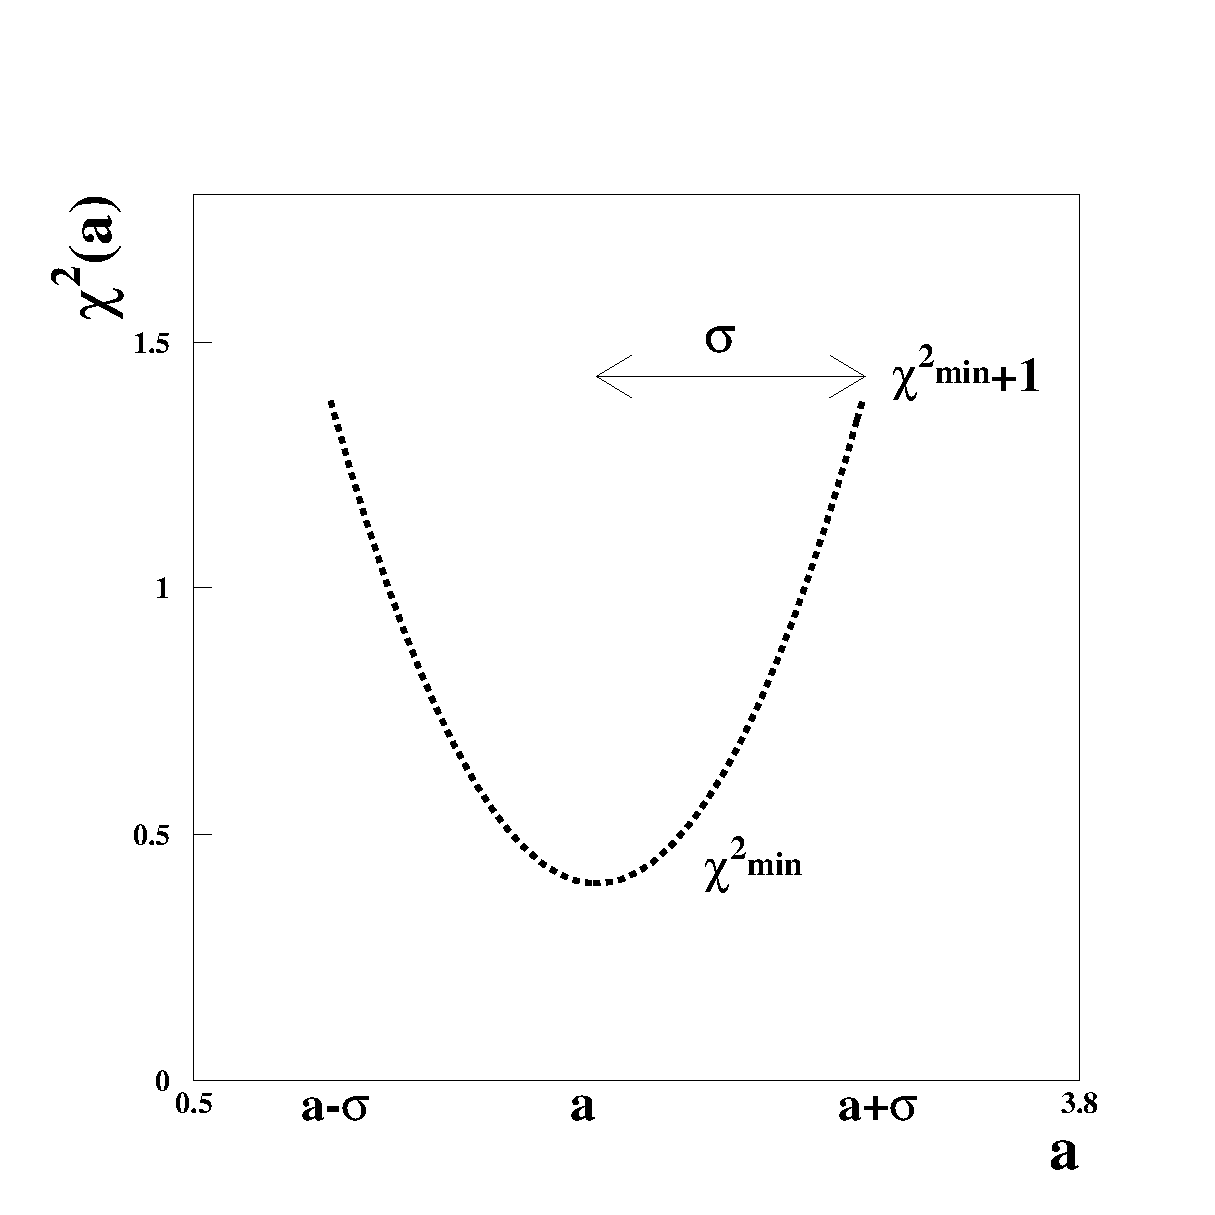
\epsfig{file=feynman/chisqp2.epsi,width=8.cm}}
     \put(8.,5.5){
\begin{minipage}[t]{7cm} 
$\rightarrow$ Read error directly\\ 
from $\chi^2$ curve
\end{minipage}
}
%    \put(8.,5.){\LARGE $\chi^2(\hat{a}+\sigma_{\hat{a}}) = 1$}
\end{picture}
\end{figure}
\vfill
\end{slide}

%
\begin{slide}
\pagestyle{headings}
\sf
\bheader{{\normalsize \bf \darkgreen Mini-exercise} Averaging of two meas. via $\chi^2$ parabolas}
%
%\large 
%Two measurements 
%$y_1$, $y_2$  of the same quantity $a$ can be represented 
%by their $\chi^2$ parabolas:
%{\darkgreen \bfseries
%\begin{itemize}
%\item
%draw for the example below the total $\chi^2$, i.e. the sum
%of the two parabolas {\red (yes, doing it simply by hand :-))}
%\item
%Read off the value $\hat{a}$ (where the total $\chi^2$ is minimal)
%\item
%Estimate the error of $\hat{a}$ from the points where
%$\chi^2 = \chi^2_{min} + 1$ 
%\end{itemize}
%}
\begin{figure}[h]
\unitlength1cm
  \begin{picture}(15,10)
% \put(1,2.8){\epsfig{file=feynman/chisq_parabola.eps,clip=,width=8.cm}}
 \put(5.7,1.3){\epsfig{file=feynman/chisq_parabola.eps,clip=,width=9.5cm}}
 \put(7.3,3.){\large $\chi^2_1$}
 \put(7.8,5.2){\large $\chi^2_2$}
 \put(-1.3,9.3){
\begin{minipage}[t]{7.3cm}
%{\darkgreen \bfseries
\large
Two measurements 
$y_1$, $y_2$  of the same quantity $a$ can be represented 
by their $\chi^2$ parabolas:
$\chi^2_i = (y_i-a)^2/\sigma_i^2; \quad i=1,2$ 
\begin{itemize}
\item
Draw for the example on the right the total $\chi^2$, i.e. the sum
of the two parabolas {\red (yes, do it simply by hand :-))}
\item
Read off the value $\hat{a}$ (where the total $\chi^2$ is minimal)
\item
Estimate the error $\sigma_{\hat{a}}$ from the points where
$\chi^2 = \chi^2_{min} + 1$ 
\item
How much is the error $\sigma_{\hat{a}}$ reduced
compared to the errors of the two original measurements?  
%For comparison read off also the
%values $y_i$ and $\sigma_i$ for $i=1,2$ and see
%how much the error is reduced
\end{itemize}
%}
\end{minipage}
}
% \put(1,0.){\epsfig{file=kumacs/chisq_parabola.eps,clip=,width=13.cm}}
\end{picture}
\end{figure}
\end{slide}


\begin{slide}
\pagestyle{headings}
\sf
\header{Averaging several measurements}
%
%\renewcommand{\baselinestretch}{1.1}
\Large
$n$ measurements $y_i\pm \sigma_i$ of the same quantity
$a$ $\rightarrow$ what is the best way to average?
%

\noindent
(Why is $\frac{1}{n} \Sigma y_i$ not the best? $\rightarrow$
measurements with large errors get too much weight and can
spoil the average!)
%
\[ \chi^2 = \Sigma_{i=1}^n \frac{\dd (y_i -a)^2}{\sigma_i^2} \]
%
\[ \frac{d\chi^2}{da} = 0 = \Sigma_{i=1}^{n} \frac{-2 (y_i - a)}{\sigma_i^2}
 = -2 \Sigma_{i=1}^{n} \frac{y_i}{\sigma_i^2} + 
    2 a \Sigma_{i=1}^{n} \frac{1}{\sigma_i^2}
\]
%
\begin{equation}
\rightarrow \quad 
\begin{array}{|lll|}
\hline
\hat{a} & = & \Sigma_{i=1}^n \frac{\dd y_i}{\dd \sigma_i^2} /  \Sigma_{i=1}^n \frac{\dd 1}{\dd \sigma_i^2} 
\\[4mm]
\hline
\end{array}
\end{equation}
%
\end{slide}




\begin{slide}
\pagestyle{headings}
\sf
\header{Averaging several measurements}
%
\Large
$\rightarrow$ Single measurements contribute with weight 
$G_i = \frac{\dd 1}{\dd \sigma_i^2}$; 

Define $G_s:= \Sigma_{i=1}^{n} G_i;$ \hspace{5mm}
%
Hesse matrix $H = 1/2 \frac{\dd d^2\chi^2}{\dd da^2} = G_s$
%
 
\begin{equation}
\rightarrow \quad 
\begin{array}{|lll|}
\hline
\hat{a} & = & \frac{1}{\Sigma_{i=1}^n G_i}  \cdot 
\Sigma_{i=1}^n G_i y_i = \frac{1}{G_s} \cdot \Sigma_{i=1}^n G_i y_i
\\[2mm]
\hline
\end{array}
\end{equation}
%
Error on $\hat{a}$: 
%
\[ 
\begin{array}{|l|}
\hline
\sigma_{\hat{a}}^2 = \Sigma_{i=1}^n \left( \frac{\dd d\hat{a}}{\dd dy_i}\right)^2 
\cdot \sigma_i^2 = 
\Sigma_{i=1}^n \left( \frac{\dd G_i}{\dd G_s}\right)^2 
\cdot \sigma_i^2 \\
= 
\frac{\dd 1}{\dd G_s^2} \cdot \Sigma_{i=1}^n G_i = \frac{\dd 1}{\dd G_s} = 
\frac{\dd 1}{\dd \Sigma_{i=1}^n 1/\sigma_i^2} 
\\[4mm]
\hline
\end{array}
\]

In short
\[ 
\begin{array}{|l|}
\hline
\hat{a} = \frac{ \dd \Sigma_{i=1}^n y_i/\sigma_i^2}{\dd
 \Sigma_{i=1}^n 1/\sigma_i^2} \; \pm \; \frac{\dd 1}{\dd 
\sqrt{\Sigma_{i=1}^n 1/\sigma_i^2} }
\\[4mm]
\hline
\end{array}
\]
\end{slide}




\begin{slide}
\pagestyle{headings}
\sf
\header{Practical work: gain from weighted average}
A radioactive source is completely surrounded by two
hemispherical counters, one with 100\% efficiency and the other
with 10\% efficiency only. 
%
An experimenter observes within one minutes $100\pm 10$ decays
in the first counter and $9\pm 3$ in the second.
%

\noindent
Estimate the total decay rate of the source per minute
using the following two methods - compare the results and
their precision:\\[2mm]
{\bfseries  A) unweighted average:}
\begin{enumerate}
\item 
Correct for each counter the observed number for the counter inefficiency
\item
Sum the corrected numbers in both counters to the total
number of decays and determine an uncertainty using error propagation
\end{enumerate}
\vspace{2mm}
{\bfseries  B)  weighted average:}
\begin{enumerate}
\item
Assume that without any inefficiency each of the counters
has 50\% geometrical acceptance, i.e. would see half of the
decays. Determine two separate measurements of the total
decay rate by correcting for each counter the efficiency corrected
rate additionally by the geometric acceptance.
\item
Calculate the weighted mean of the two separate measurements
and an error
\end{enumerate}
%
\end{slide}


%\begin{slide}
\pagestyle{headings}
\sf
\bheader{  {\normalsize \bf \darkgreen Mini-exercise}
Gain from weighted average}
%
\large
%
Die totale Teilchenrate aus einer Quelle soll gemessen werden.
Um die Quelle herum ist ein hermetischer Detektor gebaut.
Die eine H\"alfte des Detektors misst 
\[N_1 = 100 \pm 10\]
Die andere H\"alfte des Detektors ist sehr ineffizient
und misst (effizienzkorrigiert!) 
\[N_2 = 100 \pm 100\]
%
\vspace{2mm}
{\em  \darkgreen \bfseries
Sch\"atzen Sie die Gesamtrate $N$ mit den folgenden zwei Methoden:}
\begin{enumerate}
\item
$ \hat{N} = N_1 + N_2 $
\item
Multipliziere $N_1$ und $N_2$ jeweils mit Faktor 2 
(beide H\"alften 'sehen' ja 50\%!) 
$\rightarrow$ 
separate Messungen:
\begin{itemize}
\item Erste Messung: 
$ N = 200 \pm 20 $
\item Zweite Messung
$ N = 200 \pm 200 $
\end{itemize}
$\rightarrow$ Bilde das gewichtete Mittel beider Messungen
als Sch\"atzwert $\hat{N}$.
\end{enumerate}
%
\vspace{2mm}

\begin{itemize}
\item[$\rightarrow$]
{\em \darkgreen \bfseries Bestimmen Sie f\"ur beide Verfahren den Fehler auf
$\hat{N}$ (Formeln s. Vorlesung!)}
\end{itemize} 
\end{slide}



%
%
%
\begin{slide}
\pagestyle{headings}
\sf 
\header{Lecture II on linear least square fits}
%
\Large
Contents:
\begin{itemize}
\item
Consistency of measurements $\rightarrow$
$\chi^2$ fit quality test
\item 
Outlier rejection
\end{itemize}
%
\end{slide}




\begin{slide}
\pagestyle{headings}
\sf
\header{Consistency of measurements}
\Large
Example: Two measurements $y_1$ and $y_2$ with errors
$\sigma_1$ and $\sigma_2$; the true value $a$ is known,
are the measurements consistent with $a$?:
%
\begin{figure}[h]
\unitlength1cm
  \begin{picture}(8,6.2)
    \put(0.,0.4){\epsfig{file=feynman/lco1.ps,width=5.5cm}}
    \put(8.,0.4){\epsfig{file=feynman/lco2.ps,width=5.5cm}}
    \put(1.,0.){
$\chi^2 = \frac{(y_1 - a)^2}{\sigma_1^2} + 
            \frac{(y_2 - a)^2}{\sigma_2^2} = 2$}  
\put(10.,0.){$\chi^2 = 8$}
\end{picture}
\end{figure}
%
$\rightarrow \chi^2$ is a measure of the consistency
%
%\vspace{7mm}
\end{slide}
%




\begin{slide}
\pagestyle{headings}
\sf
\header{Consistency of measurements}
\Large
\underline{Expected probability density  for 
$\vec{y} = (y_1,y_2)$  (case $a=0; \sigma_1 = \sigma_2 = \sigma$):}
\begin{figure}[h]
\unitlength1cm
  \begin{picture}(8,6.)
    \put(-.6,0.){\epsfig{file=feynman/lco3.ps,width=6.2cm}}
%\put(6.,5.){$ L(\vec{y},a) \propto
%e^{-y_1^2/2} e^{-y_2^2/2} 
%\sim e^{-\chi^2/2}
%$}
\put(5.,5.3){\Large
\begin{minipage}[t]{10cm}
\[
\begin{array}{l}
{\blue f(\vec{y})} \,  dy_1 dy_2 = 
\frac{ 1}{2\pi} e^{-y_1^2/2} e^{-y_2^2/2} \, dy_1 dy_2\\[2mm]  
= {\blue \frac{1}{2\pi} e^{-r^2/2}}\, dy_1 dy_2 \quad
\mbox{with}\; r=\sqrt{y_1^2+y_2^2}\\[4mm]
 {\blue f(r)} \, dr = \frac{2\pi r}{2\pi} r e^{-r^2/2} \, dr =  {\blue r e^{-r^2/2} }\, dr\\[4mm]
\chi^2 = r^2 \rightarrow \\[2mm] 
{\blue    f(\chi^2)} \, d\chi^2 = {\blue \frac{ 1}{2} e^{-\chi^2/2}} \, d\chi^2\\
\end{array}
\]
\end{minipage}
} 
\end{picture}
\end{figure}
\vspace*{-1mm}
$\rightarrow$ introduces $\chi^2$-distr. for $z=\chi^2$ and two 
dimensions (ndf=2):
$f(z,2) = \frac{1}{2}  e^{-z/2}$
%Trafo $L(\vec{y},a) \rightarrow$ prob. density $f(\chi^2)$\\
%General result for $n$ measurements: $\chi^2$ fct. for n-degrees of freedom
%\[ \rightarrow f(\chi^2,n) = 
%\frac{1}{\Gamma(n/2)2^{n/2}} \cdot
%(\chi^2)^{n/2-1} \cdot e^{-\chi^2/2}
%\]
%
\end{slide}


\begin{slide}
\pagestyle{headings}
\sf
\header{$\chi^2$-function for $n$ degrees of freedom}
\begin{figure}[h]
\unitlength1cm
  \begin{picture}(8,6.)
    \put(-1.3,0.){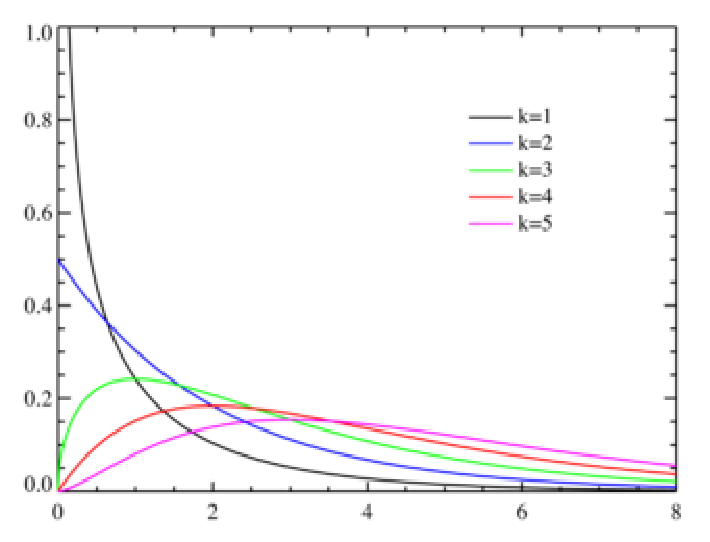
\epsfig{file=feynman/325px-Chi-square_distributionPDF.ps,
width=8.cm}}
\put(7.,5.){\Large
$f(\chi^2,n) = 
\frac{1}{\Gamma(n/2)2^{n/2}} \cdot
(\chi^2)^{n/2-1} \cdot e^{-\chi^2/2}$
}
\put(7.,4.){\Large with $\Gamma(n/2) 
= \int_{0}^{\infty} dt e^{-t} t^{n/2-1}$
}
\put(7.,3.){\framebox{
\begin{minipage}[t]{7.5cm}
\Large
%Es gilt:\\
$\int_0^{\infty} f(\chi^2,n) d\chi^2 = 1$\\[2mm]
$\langle \chi^2 \rangle = n$\\[2mm]
$V(\chi^2) = 2n; \; \sigma(\chi^2) = 
\sqrt{2n}$\\[2mm]
$\rightarrow \langle \chi^2/n \rangle = 1$\\[2mm] 
$\sigma(\chi^2/n) = \sqrt{2/n}$
\end{minipage}
}
}
\end{picture}
\end{figure}
%\vfill
%\vspace*{-5mm}
%Transformation $L(\vec{y},a) \rightarrow$ prob. density $f(\chi^2)$\\
%General result for $n$ measurements: $\chi^2$ fct. for n-degrees of freedom
%
%
\end{slide}



\begin{slide}
\Large
\pagestyle{headings}
\sf
\header{$\chi^2$-fit probability}
%
\underline{Common measure for consistency of measurements:}\\
Probability that for repeated experiments a  
$\chi^2\ge \chi^2_{actual}$ is
observed 
%
\[ prob(\chi^2,n) = \int_{\chi^2}^{\infty} f(\chi^2,n) d\chi^2
\quad \mbox{subst. } t = \chi^2/2
\]
\[ = \frac{1}{\Gamma(n/2)} \cdot \int_{\chi^2/2}^{\infty} 
dt\, e^{-t} \,t^{n/2-1} \]
%(available in CERNLIBS etc.)
%
\begin{figure}[h]
\unitlength1cm
  \begin{picture}(8,6.)
    \put(-1.3,0.){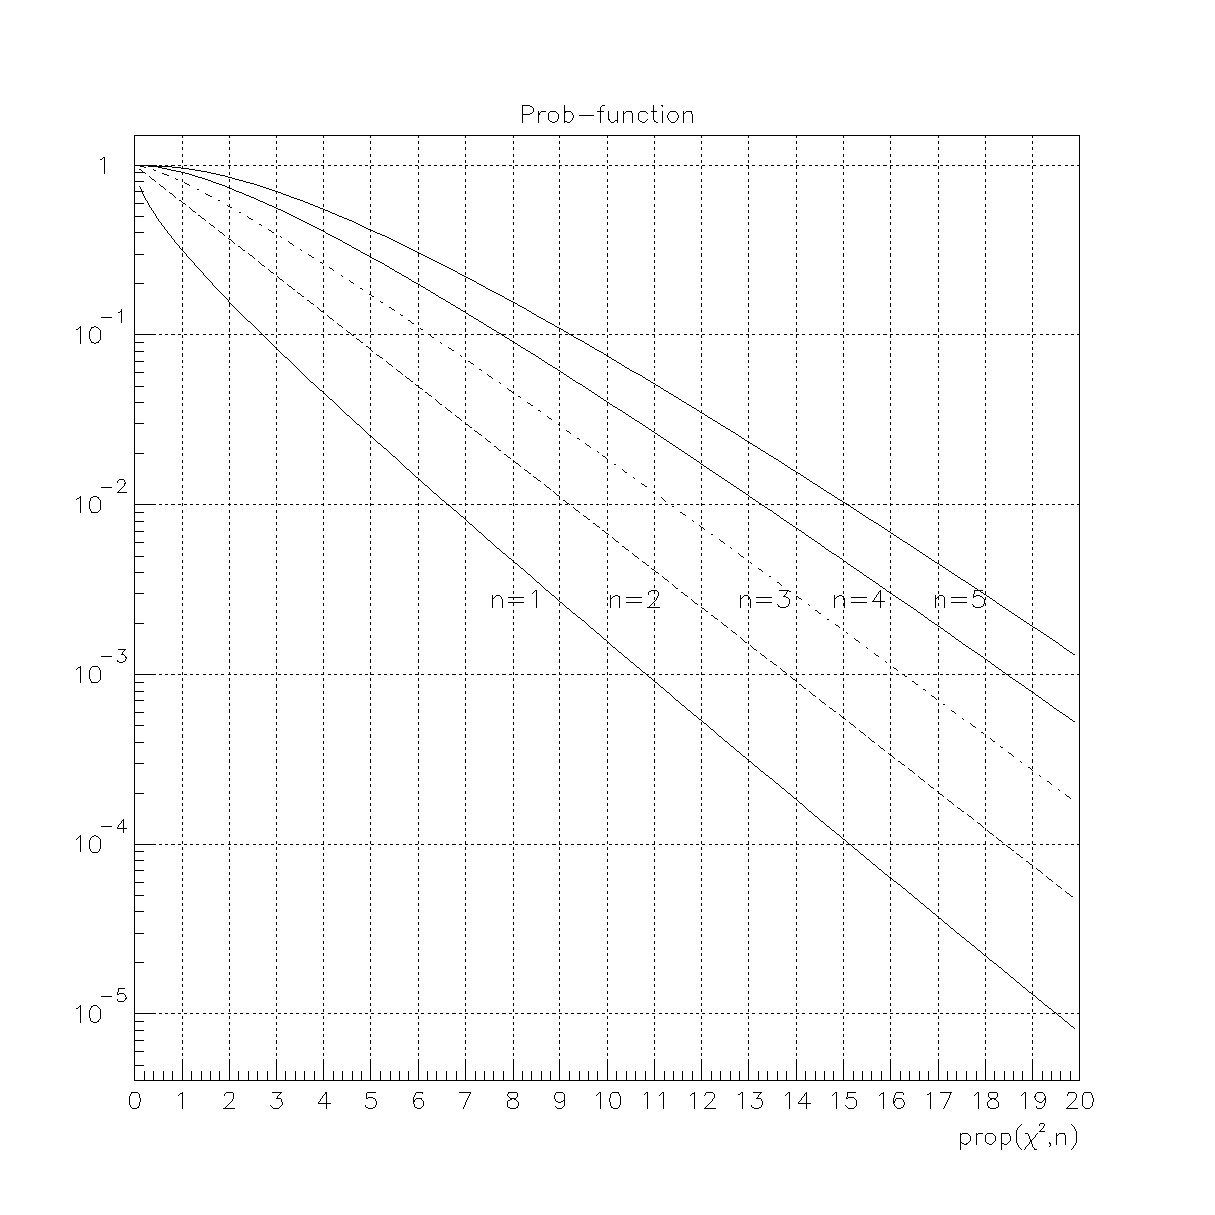
\epsfig{file=eps/probfct.eps,
width=7.cm}}
\put(-.5,1.){\large \red $prob(\chi^2,n)$ vs $\chi^2$ for various $n$}
\put(6.,3.){Add plot of expected flat distribution}
\end{picture}
\end{figure}
%
\end{slide}


\begin{slide}
\Large
\pagestyle{headings}
\sf
\header{$\chi^2$ for two measurements with unknown true value}
%
Until now the true value of $a$ was assumed to be known, 
%taken to be 
%known and used for $\chi^2$\\
%If $a$ is unknown $\rightarrow$ 
now replace by estimated $\hat{a}$;\\[2mm]
\underline{Example of two measurements:}
\begin{eqnarray*} 
\chi^2_{min} & = & 
\frac{ (y_1 - \hat{a})^2 } {\sigma_1^2} 
+
\frac{ (y_2 - \hat{a})^2 } {\sigma_2^2}
%;  
%\quad  \mbox{with} \quad G_i: = 1/\sigma_i^2 \\
\end{eqnarray*}
Using  the weighted average 
$\hat{a} = \frac{\dd G_1 y_1 + G_2 y_2}{\dd G_1+G_2}$ with $ \quad G_i: = 1/\sigma_i^2$ $\rightarrow$  
\end{slide}


\begin{slide}
\Large
\pagestyle{headings}
\sf
\header{$\chi^2$ for two measurements with unknown true value}
%
\vspace{-5mm}
\normalsize
\begin{eqnarray*}
\chi^2_{min} & = &   
  G_1 \cdot \left(y_1 - \frac{(G_1 y_1 + G_2 y_2)}{G_1+G_2} \right)^2 
+ G_2 \cdot \left(y_2 - \frac{(G_1 y_1 + G_2 y_2)}{G_1+G_2} \right)^2 \\
& = & 
  G_1 \cdot \left(\frac{(G_2 y_1 - G_2 y_2)}{G_1+G_2} \right)^2 
+ G_2 \cdot \left(\frac{(G_1 y_2 - G_1 y_1)}{G_1+G_2} \right)^2 \\
& = & 
\frac{G_1 G_2^2}{(G_1+G_2)^2} (y_1 -y_2)^2 + 
\frac{G_2 G_1^2}{(G_1+G_2)^2} (y_1 -y_2)^2 \\
& = & 
\frac{G_1 G_2 (G_1+G_2)}{(G_1+G_2)^2} \cdot  (y_1 -y_2)^2 
 =  \frac{G_1 \cdot G_2}{G_1+G_2} \cdot (y_1-y_2)^2\\ 
& = & 
\frac{1}{1/G_1 + 1/G_2} \cdot (y_1 - y_2)^2 
 = {  \pmb{  \frac{1}{\sigma_1^2+\sigma_2^2} \cdot 
(y_1-y_2)^2}} 
\end{eqnarray*}
\Large 
$\Delta = 
\frac{y_1 - y_2}{\sqrt{\sigma_1^2 +\sigma_2^2}}$ should follow
{\blue  \small \it (errorpropagation!)} 
gauss distribution $\sim e^{-\frac{\Delta^2}{2}}$\\[1mm]
$ \rightarrow$ $\chi^2 = \Delta^2$ follows \underline{1-dim} $\chi^2$
distr.!\\[1mm]
$\rightarrow$ One degree of freedom ``sacrificed'' for determination of
$\hat{a}$.\\[2mm]
\framebox{\begin{minipage}{12cm}
General: $n$-measurements with one unknown $a$\\ 
$\rightarrow$ follows $\chi^2$ distribution 
with $n-1$ degrees of freedom
\end{minipage}
}
\end{slide}


\begin{slide}
\Large
\pagestyle{headings}
\sf
\bheader{\darkgreen{Mini-exercise} Plot $\chi^2$ curves with computer}
%
\begin{figure}[h]
\unitlength1cm
  \begin{picture}(8,8.)
    \put(-1.3,0.){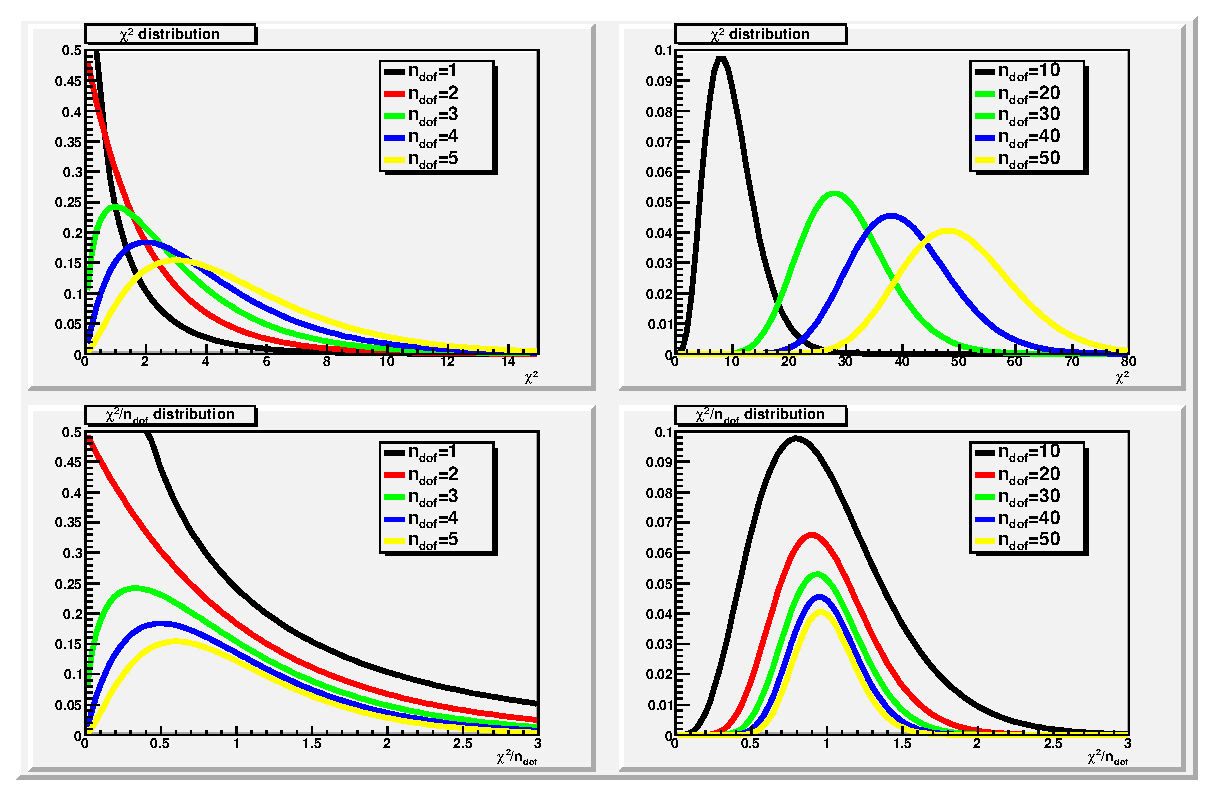
\epsfig{file=eps/chisq_ndf_curves.eps,width=12.cm}}
%    \put(-1.3,0.){\epsfig{file=prob_examples.ps,width=7.cm}}
\put(0.,-1.){\normalsize see  $/afs/desy.de/user/m/mgoebel/public/StatisticsWS/ChiSquareDistribution.C$}

%\put(-.5,1.){\large \red $prob(\chi^2,n)$ vs $\chi^2$ for various $n$}
%\put(6.,3.){Add plot of expected flat distribution}
\end{picture}
\end{figure}
%
\end{slide}

\begin{slide}
\Large
\pagestyle{headings}
\sf
\bheader{\darkgreen{Mini-exercise} Outlier rejection}
%
\begin{figure}[h]
\unitlength1cm
  \begin{picture}(8,8.)
    \put(2.,10.){\rotatebox{-90}{\epsfig{file=eps/average_mw_new.ps,width=8.cm}}}
%    \put(-1.3,0.){\epsfig{file=prob_examples.ps,width=7.cm}}

\put(0.,1.5){\normalsize see  $/afs/desy.de/user/m/mgoebel/public/StatisticsWS/AverageMW.C$}
\put(0.,1.){
\begin{minipage}[t]{14cm}
\darkgreen
Tasks: Determine weighted average, the $\chi^2_{min}$ and fit probability,
see what happens if one takes out the value with the largest deviation from the mean,
etc.
\end{minipage}
}
%\put(-.5,1.){\large \red $prob(\chi^2,n)$ vs $\chi^2$ for various $n$}
%\put(6.,3.){Add plot of expected flat distribution}
\end{picture}
\end{figure}
%
\end{slide}

%
%
%
\begin{slide}
\pagestyle{headings}
\sf 
\header{Lecture III on linear least square fits}
%
\Large
Contents:
\begin{itemize}
\item
General solution (normal equations)
of linear least square fits
\item 
Straight line fits ... and other fit examples
\end{itemize}
%
\end{slide}




\begin{slide}
\Large
\pagestyle{headings}
\sf
\header{Solution via normal equations}
Linear fit $\rightarrow$ determines estimator for $\vec{a}$
\[ \chi^2 = (\vec{y} - A\vec{a})^{t} V^{-1} 
            (\vec{y} - A\vec{a}) \]
\[Min. \chi^2 \;\rightarrow \;\frac{d\chi^2}{d\vec{a}^{\,t}}  = 0 \]
\[ \rightarrow \;-2 A^t V^{-1} (\vec{y} - A \vec{a}) = 0
\]
\[ \rightarrow \; A^t V^{-1} A \vec{a} = A^{t} V^{-1} \vec{y} \]

\noindent
{\em Side remark: why can't we just set: 
$\vec{y} = A \vec{a}$ ??? Because 
$\vec{y}$ has dimension
$n$ and $\vec{a}$ has dimension $m$ !!!
}
\noindent
\underline{Solution:}
\[ 
\begin{array}{||lll||} 
\hline
\hline
\vec{a} &  = &   (A^t V^{-1} A)^{-1} A^t V^{-1} \vec{y}  \\
 & = & H^{-1} A^t V^{-1} \vec{y} \\
 & = & U A^t V^{-1} \vec{y} \\
 & & \mbox{with}\; U= H^{-1} = Cov(a) \\ 
\hline
\hline
\end{array}
\quad
\mbox{\blue \em Normal equations}
\]
%
%
\end{slide} 


%%%% skip \begin{slide}
\pagestyle{headings}
\sf
%
\header{To be xchecked: Properties of linear least square fits}
%
\large 
\sf
\begin{enumerate}
\item 
\underline{consistency:} $\lim_{N\rightarrow \infty } \hat{\vec{a}} = \vec{a}$
\hspace{1cm} (follows from next point)
%$  \hspace{5mm}  ($\hat{\vec{a}} = B \vec{y}$  
%und $\vec{y}$ konvergiert
%) 
\item 
\underline{Unbiasedness}: 
$\langle \hat{\vec{a}} \rangle = 
\langle B \vec{y} \rangle = 
B\, \langle \vec{y} \rangle = 
B \,A \,\vec{a} = 
(A^t\, V^{-1}\, A)^{-1}  \,A^t \,V^{-1}\, A \,\vec{a} = \vec{a}
$\\
$\rightarrow$ unbiased!
\item \underline{Efficiency:} Gauss-Markov-Theorem: \\[2mm]
\framebox{\begin{minipage}{14cm}
For randomly distributed $\vec{y}$ 
the linear least square fit is the most 
efficient  estimator
\end{minipage}
}

{\normalsize(Proof e.g. in Blobel/Lohrmann book)}
%
\item 
%\underline{and}:
For measurements $\vec{y}$ with gaussian errors and if
$\vec{y} = A \vec{a}$ is the correct model,
then $\chi^2$ follows 
a $\chi^2$-distribution with 
N-m degrees of freedom 
(with N  = number of data points and m = number of fit parameters)
\end{enumerate}
%
\end{slide}

\begin{slide}
\pagestyle{headings}
\sf
%
\vspace*{-4mm}
\header{Straight line fit}
\vspace{5mm}
\Large 
\sf
\begin{figure}[h]
\unitlength1cm 
  \begin{picture}(8,5.)
    \put(7.,-1.){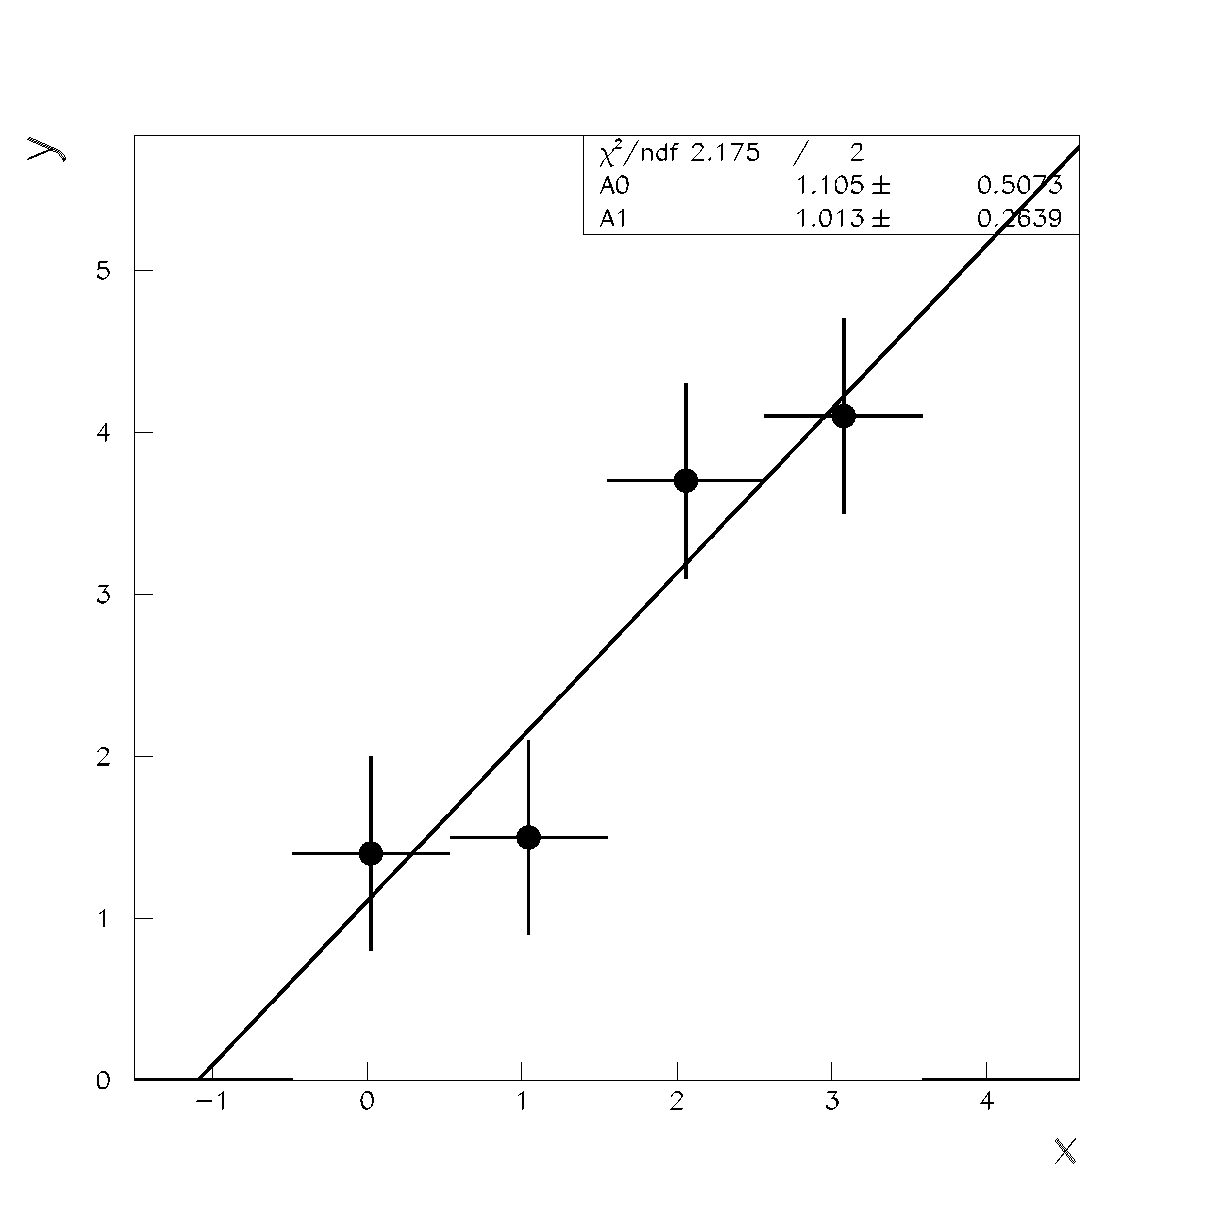
\epsfig{file=eps/p1.eps,width=7.cm}}
\put(0.,2.5){
\begin{minipage}{6.3cm}
\large \sf
{\bfseries Model: $\pmb{y = a_0 + a_1 x }$}\\[1mm]
Simple example: All $y_i$ have the same uncertainty and
are uncorrelated
\[  
V = \left(
\begin{array}{lll}
\sigma^2 &    &    0 \\
         & .  &      \\
0        &    &    \sigma^2 \\
\end{array}
\right) 
 \]
\[ \chi^2 = \sum_{i=1}^n \frac{\dd (y_i - a_0 - a_1\, x_i)^2}{\dd \sigma^2} \]

\end{minipage}
}
\end{picture}
\end{figure}


\large \sf
\vspace{4mm}

Matrix notation: $ \vec{y} = A\vec{a}; \qquad 
\vec{a} 
\left(
\begin{array}{l}
a_0\\
a_1\\
\end{array}
\right)
\quad
A = 
\left( 
\begin{array}{ll}
  1 & x_1 \\
  . & .   \\
  1 & x_n \\
 \end{array}
\right)
, \quad 
A^T = 
\left(
\begin{array}{lll}
    1 & ... & 1   \\
  x_1 & ... & x_n \\
\end{array}
\right)
$
\begin{eqnarray*} 
 \hat{\vec{a}} & =  & \left( 
\begin{array}{l}
\hat{a}_0 \\
\hat{a}_1 \\
 \end{array}
\right)
= ( A^T V^{-1} A )^{-1} A^T V^{-1} \vec{y}
; \qquad V^{-1} = 
\left(
\begin{array}{lll}
1/\sigma^2 &    &    0 \\
         & .  &      \\
0        &    &    1/\sigma^2 \\
\end{array}
\right) 
\\
\end{eqnarray*}
\end{slide}
%
%
%
\begin{slide}
\pagestyle{headings}
\sf
%
\header{Straight line fit}
%\vspace*{-5mm}
\begin{eqnarray*} 
 \hat{\vec{a}} 
 &  = &  \sigma^2 ( A^T A)^{-1} \cdot \frac{1}{\sigma^2} A^T\cdot \vec{y} 
\;  = \; (A^T A)^{-1} A^T \cdot \vec{y} 
\\
&  = & \left(
\begin{array}{ll}
\sum_{i} 1 & \sum_{i} x_i \\
. & . \\
\sum_{i} x_i & \sum_{i} x_i^2 \\
\end{array}
\right)^{-1} \cdot 
\left( 
\begin{array}{l}
\sum_{i} y_i \\
\sum_{i} x_i y_i \\
\end{array}
\right)
\; 
 =\;  \left(
\begin{array}{ll}
N & N \overline{x} \\
N \overline{x} & N \overline{x^2} \\
\end{array}
\right)^{-1} 
\cdot \left( 
\begin{array}{l} 
N\overline{y} \\
N\overline{xy} \\
\end{array}
\right) 
\\
&  =  & \left(
\begin{array}{ll}
1 & \overline{x} \\
\overline{x} & \overline{x^2} \\
\end{array}
\right)^{-1} \cdot 
\left( 
\begin{array}{l} 
\overline{y}\\
\overline{xy}\\
\end{array}
\right)
\; 
 = 
\; 
\frac{1}{\overline{x^2} - \overline{x}^2} 
\left(
\begin{array}{lr} 
\overline{x^2} & -\overline{x} \\
-\overline{x} & 1 \\
\end{array}
\right) 
\left( \begin{array}{l}
\overline{y}\\
\overline{xy} 
\end{array}
\right) 
%\\[4mm]
%&  = &  
= 
\frac{1}{V[x]} \cdot
\left( 
\begin{array}{l} 
\overline{x^2} \overline{y} - \overline{x}\, \overline{xy} \\
-\overline{x}\,\overline{y} + \overline{xy} \\
\end{array}
\right) 
\end{eqnarray*}
Covariance matrix:
\[ \pmb{U} = \left(
\begin{array}{ll}
\sigma_{a_0}^2 & cov(a_0,a_1) \\
cov(a_0,a_1) & \sigma_{a_1}^2 \\
\end{array}
\right)  = (A^t V^{-1} A )^{-1} = \pmb{\frac{\sigma^2}{N V[x]} 
\left( \begin{array}{lr}
\overline{x^2} & -\overline{x} \\
-\overline{x} & 1 \\
\end{array}
\right) 
}
\]
\end{slide}

%\vspace{2mm}
\begin{slide}
\Large
\pagestyle{headings}
\sf
\bheader{Mini exercise: straight line track-fit with N detectors}
%\renewcommand{\baselinestretch}{0.4}
%{\bfseries 
\noindent
The covariance formula 
\[ 
 \left(
\begin{array}{ll}
\sigma_{a_0}^2 & cov(a_0,a_1) \\
cov(a_0,a_1) & \sigma_{a_1}^2 \\
\end{array}
\right) = 
\frac{\sigma^2}{N V[x]}
\left( \begin{array}{lr}
\overline{x^2} & -\overline{x} \\
-\overline{x} & 1 \\
\end{array}
\right) 
\]
is valid for e.g. a straight line track fit  
in N detectors of resolution $\sigma$:

{
\darkgreen 
\bfseries \large
 Determine  
the improvements on the slope error  $\pmb{\sigma_{a_1}}$
by:
\begin{itemize}
\item[a)] 
Doubling the number of detector layers\\ within the same interval
in $\pmb{x}$
\item[b)] Distributing the detector layers\\ over an interval in
$\pmb{x}$ twice as large
\item[c)] 
Buying detectors with measurement uncertainties\\ reduced by a factor two
\end{itemize}
}
\end{slide}


\begin{slide}
\Large
\pagestyle{headings}
\sf
\bheader{\darkgreen{Mini-exercise} Straight-line fit example}
%
\begin{figure}[h]
\unitlength1cm
  \begin{picture}(8,8.)
    \put(0.,0.){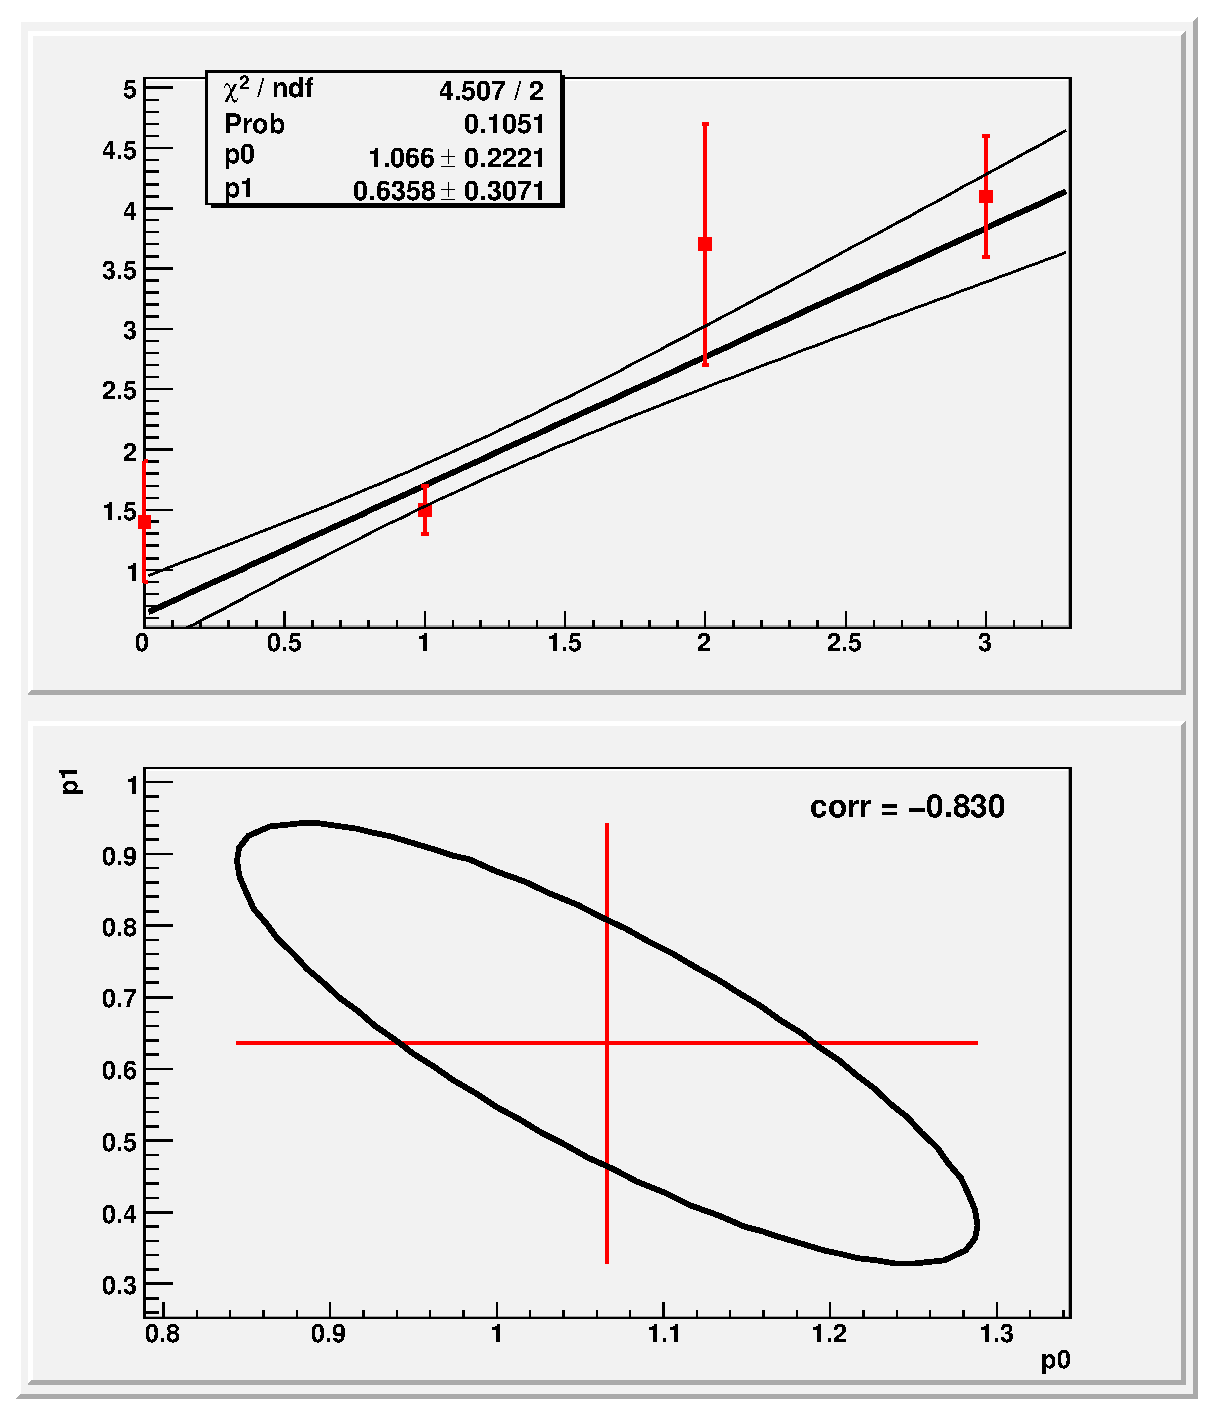
\epsfig{file=eps/straightline.eps,width=7.cm}}
%    \put(-1.3,0.){\epsfig{file=eps/prob_examples.ps,width=7.cm}}

\put(0.,-1.){\normalsize see  $/afs/desy.de/user/m/mgoebel/public/StatisticsWS/StraightLineFit.C$}
\put(8.,7.){
\begin{minipage}[t]{7cm}
\darkgreen

Tasks: Do the fit, plot the error ellipse, get the 1-sigma band, judge
fit quality, etc. 
\end{minipage}
}
%\put(-.5,1.){\large \red $prob(\chi^2,n)$ vs $\chi^2$ for various $n$}
%\put(6.,3.){Add plot of expected flat distribution}
\end{picture}
\end{figure}
%
\end{slide}

\begin{slide}
\Large
\pagestyle{headings}
\sf
\bheader{\darkgreen{Mini-exercise} Real Trackfit in Si + driftchamber}
\vspace{4mm}
%
\begin{figure}[h]
\unitlength1cm
  \begin{picture}(8,8.)
    \put(-1.5,-1.){\epsfig{file=eps/trackfit.ps,width=10.cm}}
%    \put(-1.3,0.){\epsfig{file=eps/prob_examples.ps,width=7.cm}}
%\put(0.,-1.){\normalsize see  $/afs/desy.de/user/m/mgoebel/public/StatisticsWS/StraightLineFit.C$}
\put(8.,7.){
\begin{minipage}[t]{7cm}
\darkgreen

Tasks: Do the straight line fit, plot the error ellipse, get the 1-sigma band, judge
fit quality, reject outliers!, fit with parabola, determine momentum and error, 
extension: add vertex constraint 
\end{minipage}
}
%\put(-.5,1.){\large \red $prob(\chi^2,n)$ vs $\chi^2$ for various $n$}
%\put(6.,3.){Add plot of expected flat distribution}
\end{picture}
\end{figure}
%
\end{slide}

%\begin{slide}
\pagestyle{headings}
\sf
%\darkgreen
%
\bheader{{\normalsize \darkgreen Mini-exercise:} Find best data parametrisation}
%
\Large
The plots on the next two pages show  
$\chi^2$-fits of the same data distribution
with eight different 
parametrisations (polynomials of different orders).
%
Which parametrisation is the most reasonable one?
Try to judge using  the following three criteria:
\begin{enumerate}
\item 
optically, how well the curves fit the data
\item
 a reasonable parametrisation should lead to
$\chi^2/ndf \approx 1$.
\item
choose only a more complicated parametrisation if
a significant improvement of $\chi^2/ndf$ can be achieved
\end{enumerate}
$\rightarrow$ 
Try to find your personal favorite.
\end{slide}

\begin{slide}
\pagestyle{headings}
\sf
%
\bheader{{\normalsize \darkgreen Mini-exercise:} Find best data parametrisation}
\large
\begin{center}
\begin{figure}[h]
\unitlength1cm
  \begin{picture}(15,11.)
 \put(0.,0){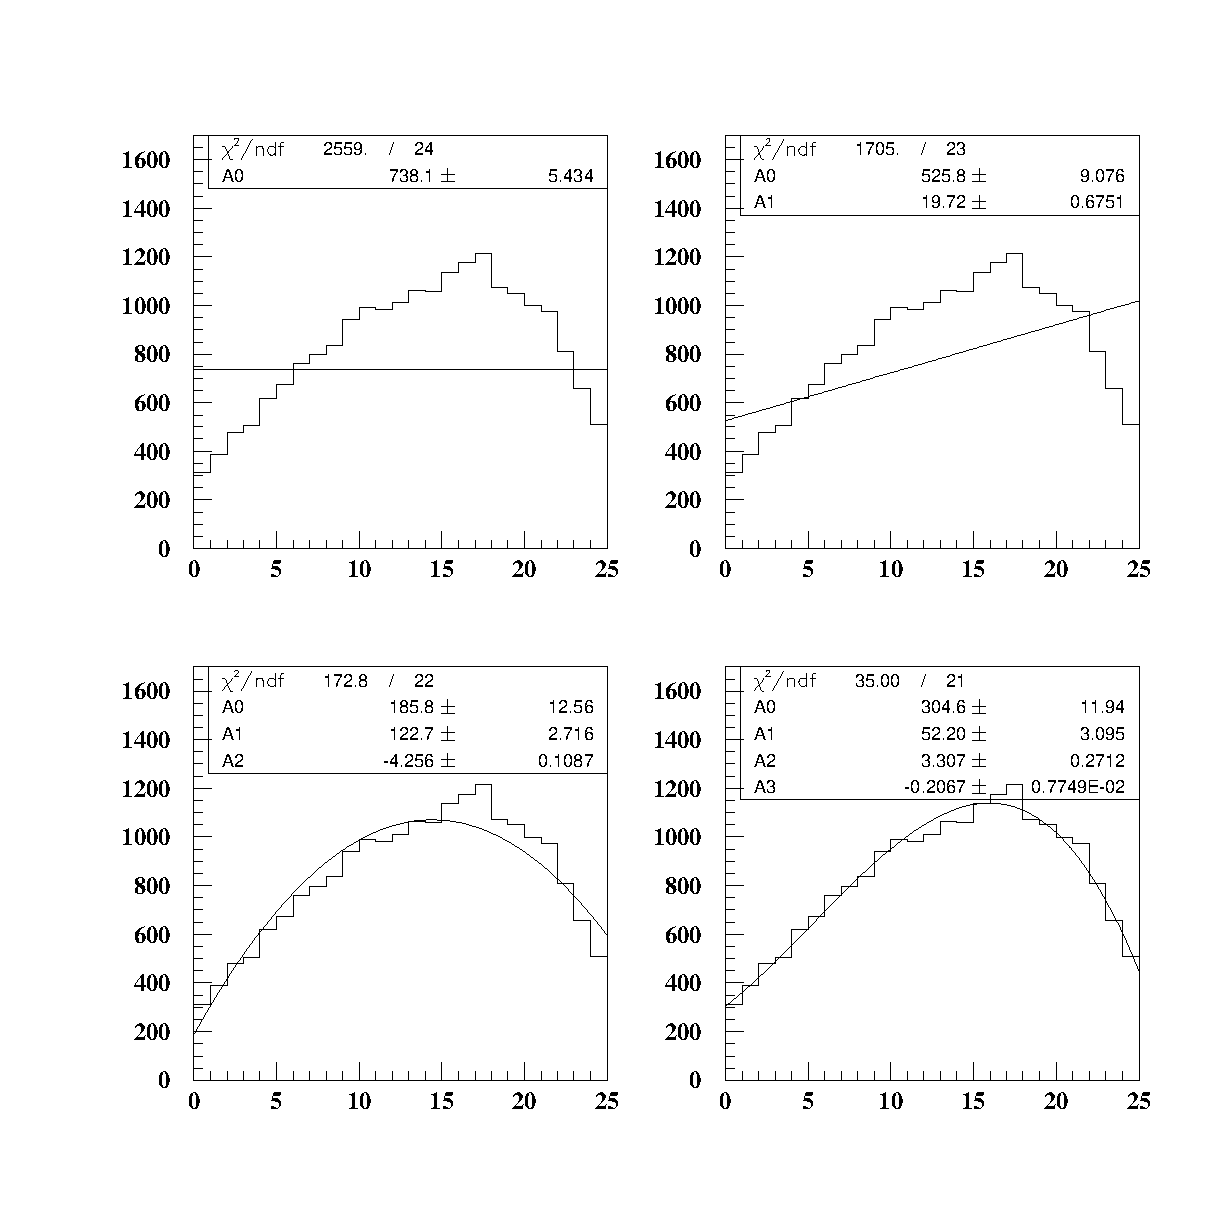
\epsfig{file=eps/p4_page1.eps,clip=,width=12.cm}}
\end{picture}
\end{figure}
\end{center}
\end{slide}

\begin{slide}
\pagestyle{headings}
\sf
%
\bheader{{\normalsize \darkgreen Mini-exercise:} Find best data parametrisation}

\large
\begin{center}
\begin{figure}[h]
\unitlength1cm
  \begin{picture}(15,11.)
 \put(0.,0){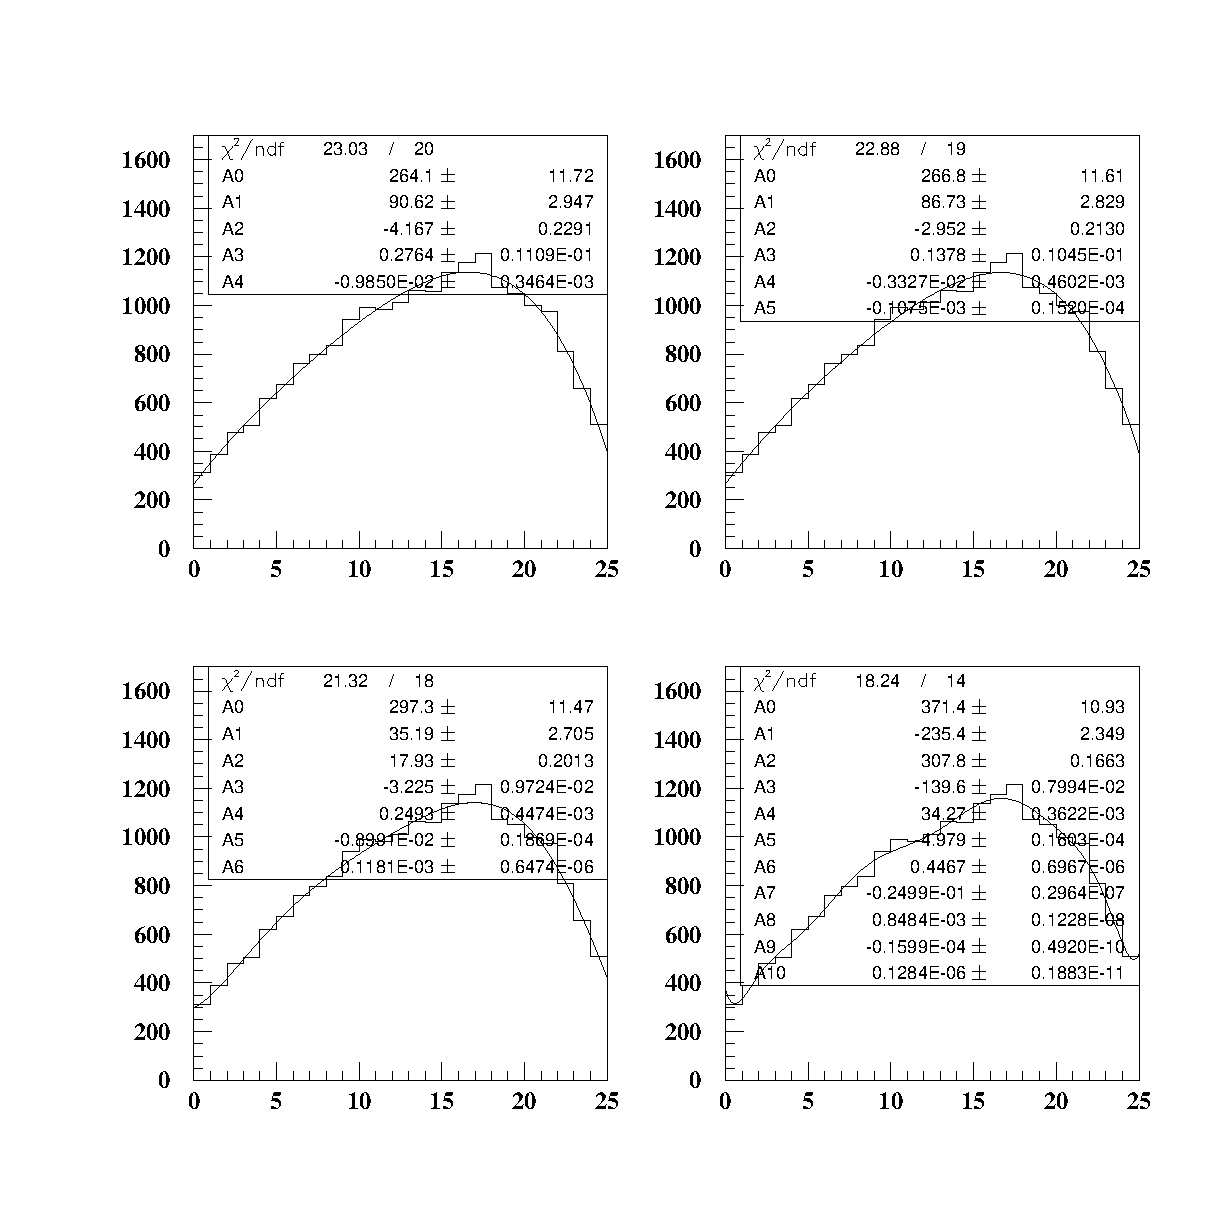
\epsfig{file=eps/p4_page2.eps,clip=,width=12.cm}}
\end{picture}
\end{figure}
\end{center}

\end{slide}

\end{document}
%
